\documentclass[preprint,12pt,number]{elsarticle}

\usepackage[utf8]{inputenc}
\usepackage[T1]{fontenc}
\usepackage{amsmath,amssymb}
\usepackage{graphicx}
\usepackage{booktabs}
\usepackage{siunitx}
\usepackage{hyperref}
\usepackage{algorithm}
\usepackage{algorithmic}
\usepackage{multirow}
\usepackage{textcomp}

\graphicspath{{figures/}}

\journal{Engineering Applications of Artificial Intelligence}

\begin{document}

\begin{frontmatter}

\title{Automated Indoor CFD Analysis from a Single 2D Image via Vision-Language Model Abstraction}

\author[kier,ust]{Younghwan Joo}
\ead{yhjoo@kier.re.kr}
\address[kier]{Energy Efficiency Research Division, Korea Institute of Energy Research, 152 Gajeong-ro, Yuseong-gu, Daejeon 34129, Republic of Korea}
\address[ust]{Energy Engineering, University of Science \& Technology, 217 Gajeong-ro, Yuseong-gu, Daejeon 34129, Republic of Korea}

\begin{abstract}
CFD simulation of indoor environments requires three-dimensional geometric models that take hours to days of manual effort to construct. This paper presents a framework that converts a single 2D image of an indoor space into a steady-state CFD solution by using a vision-language model (VLM) as the geometric abstraction engine. Given an architectural drawing or rendered image, the VLM (Gemini 3.1 Pro) extracts a structured 3D scene description (room geometry, internal obstacles, and ventilation openings), which is then scale-calibrated using one reference dimension and automatically meshed and solved with OpenFOAM. A rule-based benchmark of 20 indoor geometries at four complexity levels and five input view types (100 cases total) provides independently computed reference CFD solutions with no VLM involvement in the ground truth. Of 100 cases, 97 converge; the framework achieves a mean structural score of 0.781 and a mean CFD agreement score of 0.477. Floor-plan inputs perform best (structural 0.884, CFD 0.572); section views perform worst (0.679, 0.396). Room topology is correctly identified in 95\% of cases, and opening-wall assignment matches the reference in 70\% overall (100\% for floor plans). Three failure modes are identified: composite-room collapse under section views, obstacle hallucination with limited CFD penalty, and a structure-versus-fidelity gap in dense configurations. The pipeline, benchmark, and evaluation code are publicly available.
\end{abstract}

\begin{keyword}
indoor CFD \sep vision-language model \sep geometric abstraction \sep automated simulation \sep benchmark
\end{keyword}

\end{frontmatter}

\section{Introduction}
\label{sec:introduction}


\subsection{Motivation}
\label{sec:motivation}


Manufacturing facilities account for a large share of total energy consumption in industrialised economies, and governmental carbon-reduction targets are driving systematic energy audits across sectors \cite{gourlis.kovacic2017BuildingInformation,zhao.etal2021IndustrialReheating}. Indoor airflow patterns within factories, warehouses, and processing halls directly affect HVAC energy consumption, process thermal management, and worker thermal comfort. CFD simulation can reveal recirculation zones, thermal stratification, short-circuiting of supply air, and other phenomena that point measurements miss and energy consumption data alone cannot explain \cite{vuorinen.etal2020ModellingAerosol,liu.etal2019ReviewCFD}.

Despite its diagnostic value, CFD-based airflow analysis is rarely included in standard energy audit workflows. The barrier is not the simulation itself (modern solvers such as OpenFOAM \cite{weller.etal1998TensorialApproach} handle typical indoor geometries in minutes to hours) but the upstream geometry preparation step. Converting site photographs or architectural drawings into a CFD-ready 3D model requires CAD expertise and several hours to days of modelling work unavailable within standard audit budgets \cite{calzolari.liu2021DeepLearning}, effectively excluding CFD from the energy diagnostician's toolkit.

Existing approaches have not fully resolved this bottleneck. BIM-to-CFD workflows \cite{utkucu.sozer2020InteroperabilityData,weerasuriya.etal2019HolisticFramework,hou.etal2022PredictionOptimization} require a digital building model that rarely exists for older industrial facilities \cite{gourlis.kovacic2017BuildingInformation}. Scan-to-BIM methods \cite{rocha.etal2020ScantoBIMMethodology} demand specialised equipment impractical during a time-constrained site visit. Deep-learning surrogates \cite{guo.etal2016ConvolutionalNeural,calzolari.liu2021DeepLearning,kastner.dogan2023GANBasedSurrogate} are limited to pre-trained geometry families and cannot handle diverse industrial layouts.

An energy diagnostician who could photograph a facility space, or use an existing floor plan, and obtain a CFD-quality airflow assessment within minutes, without manual geometry modelling, would bypass this bottleneck entirely. Vision-language models (VLMs) with spatial reasoning capabilities \cite{openai.etal2023GPT4Technical,geminiteam.etal2023GeminiFamily,chen.etal2024SpatialVLMEndowing,hong.etal20233DLLMInjecting} now offer a path toward this goal. A VLM can interpret a photograph or architectural drawing, extract the spatial layout including dimensions and major obstacles, and express this information in a structured format that can be automatically converted into a CFD-ready mesh.

This paper presents and evaluates such a framework. The current implementation and benchmark use general indoor spaces rather than industrial facilities, because the simpler case permits a controlled benchmark with well-defined complexity levels. The methodology itself, VLM-based geometric abstraction from a single 2D image followed by automated CFD, applies equally to industrial spaces.

\subsection{Related work}
\label{sec:related-work}


\textbf{CFD for indoor environmental analysis.} CFD simulation of indoor environments covers ventilation effectiveness \cite{kosutova.etal2019CrossventilationGeneric,liu.etal2019ReviewCFD}, thermal comfort \cite{chen.etal2021UnsteadystateCFD}, contaminant and pathogen dispersion \cite{vuorinen.etal2020ModellingAerosol,liu.etal2021SimulationbasedStudy,srivastava.etal2021EffectiveVentilation}, and building energy performance \cite{brozovsky.etal2022AssessingImpact,ren.cao2019DevelopmentApplication}. In industrial contexts (furnaces \cite{zhao.etal2021IndustrialReheating}, process ventilation, occupational exposure), use remains far less systematic than in commercial building design, largely due to the geometry preparation overhead.

\textbf{Geometry acquisition and the automation gap.} BIM platforms can export geometry to CFD tools \cite{utkucu.sozer2020InteroperabilityData,hou.etal2022PredictionOptimization}, but BIM penetration in the industrial sector is limited \cite{gourlis.kovacic2017BuildingInformation}. Scan-to-BIM methods \cite{rocha.etal2020ScantoBIMMethodology,wang.etal2019ApplicationOriented} produce detailed as-built models from point clouds but are prohibitive for routine energy audits. Image-based reconstruction methods including NeRF \cite{mildenhall.etal2020NeRFRepresenting} yield implicit or noisy representations that cannot be directly used by finite-volume solvers, a fundamental mismatch with CFD input requirements.

\textbf{Data-driven flow prediction.} Neural network surrogates \cite{guo.etal2016ConvolutionalNeural,calzolari.liu2021DeepLearning,kastner.dogan2023GANBasedSurrogate} are fast but are limited to their training domain and cannot provide the conservation guarantees of physics-based solvers, making them unsuitable for liability-sensitive engineering assessments.

\textbf{LLM-assisted CFD workflows.} FLUID-GPT \cite{yang.etal2023FLUIDGPTFast} used a generative transformer as a CFD surrogate for erosion prediction. OpenFOAMGPT \cite{pandey.etal2025OpenFOAMGPTRetrievalaugmented} and Dong et al. \cite{dong.etal2025FinetuningLarge} automated solver configuration through LLM agents. All three address the \textit{downstream} workflow (solver setup, parameter selection, result interpretation) while assuming the geometric model already exists. The \textit{upstream} problem of extracting geometry from visual input remains open.

\textbf{Vision-language models for spatial understanding.} VLMs such as GPT-4 \cite{openai.etal2023GPT4Technical} and Gemini \cite{geminiteam.etal2023GeminiFamily} can localise objects, estimate dimensions, and interpret scene layouts \cite{chen.etal2024SpatialVLMEndowing,hong.etal20233DLLMInjecting}. The present work uses these capabilities not to reconstruct scene geometry in full fidelity, but to abstract it into a simulation-compatible schema: topological correctness and approximate dimensions rather than surface-level detail.

\subsection{Contributions}
\label{sec:contributions}


This paper contributes the following:

1. An automated image-to-CFD framework that eliminates the manual geometry preparation step by using a VLM to extract a simulation-ready 3D scene description from a single 2D image, targeting screening-level indoor airflow analysis.
2. A systematic benchmark comprising 100 evaluation cases (20 geometries $\times$ 5 view types) with independently computed reference CFD solutions, providing the first quantitative assessment of VLM-based geometric abstraction for downstream CFD accuracy.
3. An evaluation methodology that decouples geometric fidelity from flow-field accuracy, revealing that structural similarity does not guarantee CFD agreement, a finding with practical implications for acceptable error thresholds in screening applications.
4. Identification of three characteristic failure modes (composite-room collapse, obstacle hallucination, structure-versus-fidelity gap) that define the current performance boundary.


\section{Methodology}
\label{sec:methodology}


\subsection{Framework overview}
\label{sec:framework-overview}


The proposed framework accepts a single 2D image of an indoor space and produces a steady-state CFD solution through a five-stage pipeline Fig.~\ref{fig:method-framework}. In the first stage, the image is presented to a vision-language model (Gemini 3.1 Pro) (accessed via API in March 2026; model identifier `gemini-3.1-pro-preview`) together with a structured prompt that requests a JSON description of the room geometry, internal obstacles, and ventilation openings. The prompt specifies the coordinate system convention, unit system, and the required schema fields, but does not provide any ground-truth information about the scene. The VLM returns a scene description conforming to the `indoor\_cfd\_scene\_v1` schema, which encodes the room as one or more axis-aligned rectangular blocks, each obstacle as an axis-aligned bounding box, and each opening as a wall-anchored rectangular patch with an associated type (inlet or outlet).

\begin{figure*}[htbp]
\centering
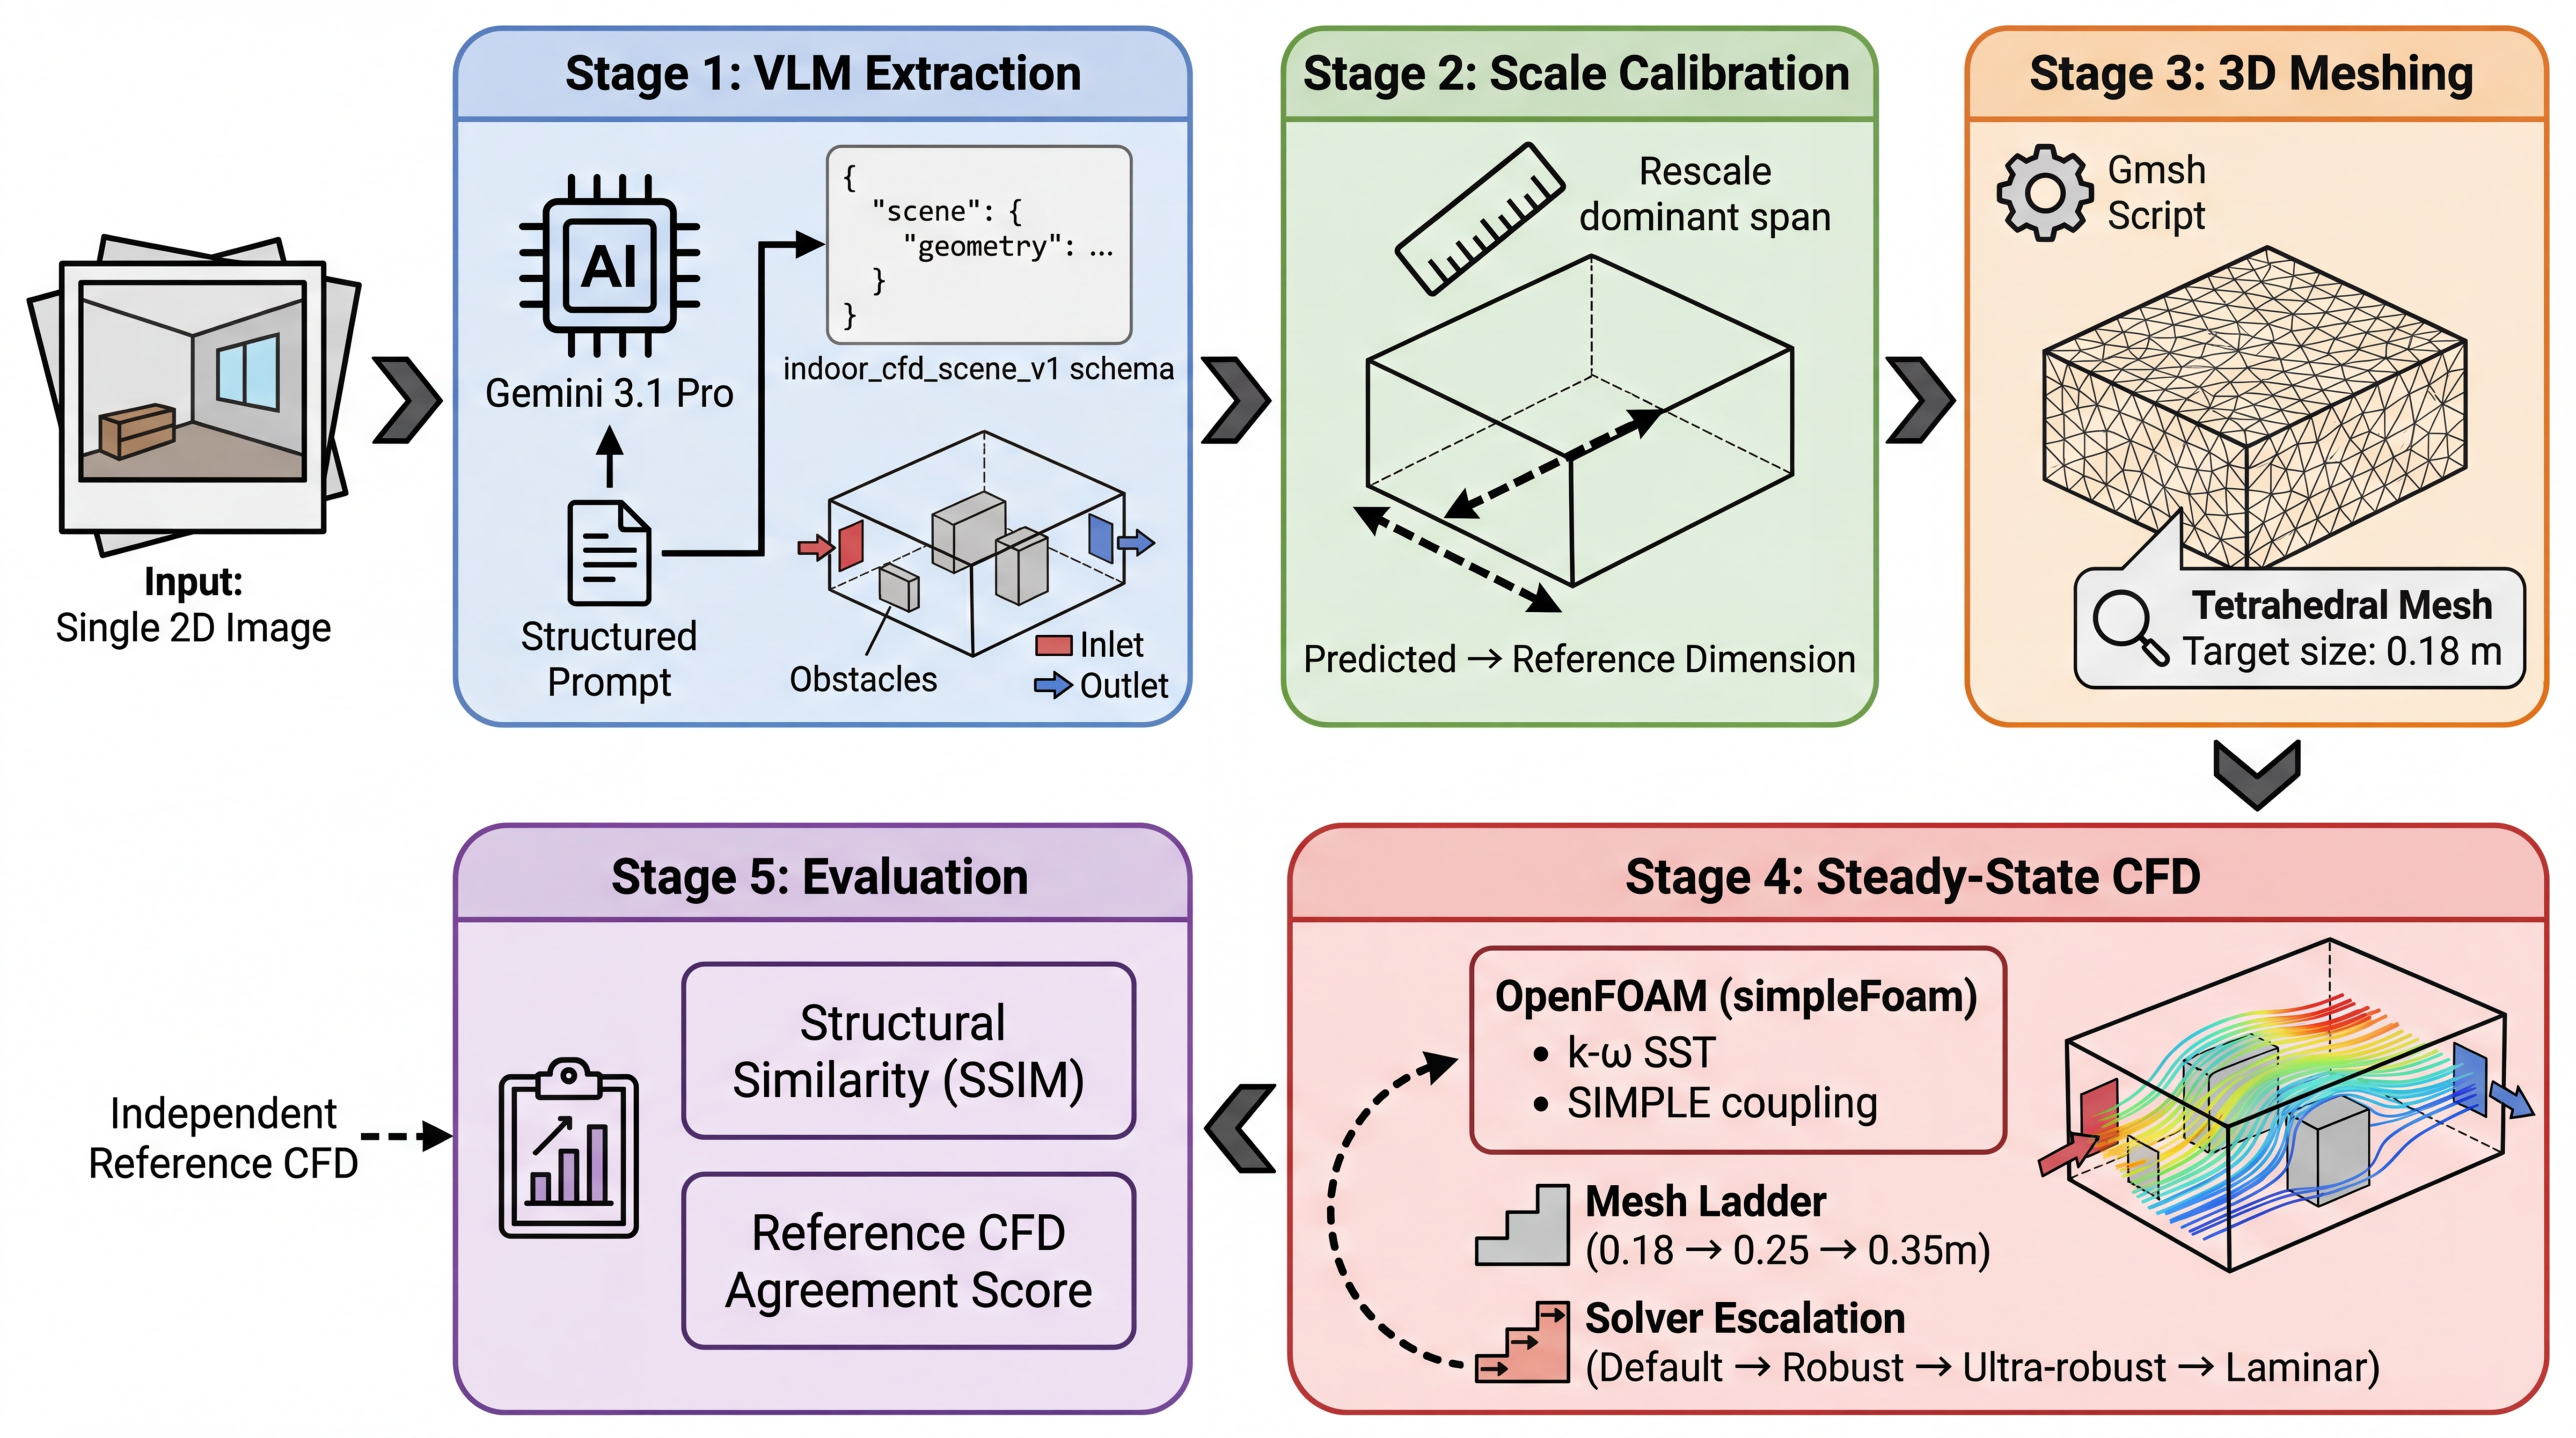
\includegraphics[width=\textwidth]{fig_method_framework}
\caption{Overall framework architecture. A single 2D image is processed by Gemini 3.1 Pro to produce a structured 3D scene description; post-hoc scale calibration corrects the dominant dimensional error using the longest horizontal span; the calibrated scene is automatically converted to an OpenFOAM case. An independent reference path generates the ground-truth CFD solution from the rule-based benchmark without VLM involvement.}
\label{fig:method-framework}
\end{figure*}

In the second stage, a single-factor scale calibration is applied to the VLM output. A single monocular image contains no absolute dimensional information; the VLM can recover proportions but not physical size. This is a fundamental limitation of any single-image approach, not a deficiency of the VLM. To obtain physically meaningful CFD results, the user provides one reference dimension, in practice a single tape-measure reading or a dimension annotation on an architectural drawing. The calibration rescales the entire scene uniformly so that the longest horizontal span matches this reference:

\begin{equation}
\alpha = \frac{L_\text{ref}}{L\_\text{pred}}, \qquad \mathbf{x}\_\text{calibrated} = \alpha \, \mathbf{x}\_\text{pred}
\label{eq:scale-calibration}
\end{equation}

where $L_\text{ref}$ is the user-provided reference span (or, in the benchmark evaluation, the corresponding ground-truth span), $L_\text{pred}$ is the longest horizontal span in the VLM prediction, and $\alpha$ is the uniform scaling factor applied to all coordinates. This single measurement is the only external input required beyond the image itself. In the benchmark, the reference span is taken from the ground-truth geometry to isolate the effect of proportional accuracy from absolute scale; in deployment, this value would come from a tape measurement or drawing annotation.

\subsection{Governing equations and CFD setup}
\label{sec:governing-equations-and-cfd-setup}


The indoor airflow is modelled as steady-state, isothermal, incompressible, turbulent flow governed by the Reynolds-averaged Navier--Stokes (RANS) equations. The continuity and momentum equations are:

\begin{equation}
\nabla \cdot \mathbf{U} = 0
\label{eq:continuity}
\end{equation}

\begin{equation}
\nabla \cdot (\mathbf{U} \otimes \mathbf{U}) = -\frac{1}{\rho}\nabla p + \nabla \cdot \bigl[(\nu + \nu\_t)\bigl(\nabla \mathbf{U} + (\nabla \mathbf{U})^\top\bigr)\bigr]
\label{eq:momentum}
\end{equation}

where $\mathbf{U}$ is the mean velocity vector, $p$ is the kinematic pressure (pressure divided by density), $\nu$ is the kinematic viscosity (air at 20 $^\circ$C, $\nu = 1.5 \times 10^{-5}$ m$^2$/s), and $\nu_t$ is the turbulent eddy viscosity.

Turbulence closure is provided by the $k$--$\omega$ SST model \cite{menter1994TwoequationEddyviscosity}, which blends the $k$--$\omega$ formulation near walls with the $k$--$\varepsilon$ formulation in the free stream. The transport equations for the turbulent kinetic energy $k$ and the specific dissipation rate $\omega$ are:

\begin{equation}
\nabla \cdot (\mathbf{U} k) = \nabla \cdot \bigl[(\nu + \sigma\_k \nu\_t) \nabla k\bigr] + P\_k - \beta^* k \omega
\label{eq:k-transport}
\end{equation}

\begin{equation}
\nabla \cdot (\mathbf{U} \omega) = \nabla \cdot \bigl[(\nu + \sigma\_\omega \nu\_t) \nabla \omega\bigr] + \frac{\gamma}{\nu\_t} P\_k - \beta \omega^2 + 2(1 - F\_1) \frac{\sigma_{\omega 2}}{\omega} \nabla k \cdot \nabla \omega
\label{eq:omega-transport}
\end{equation}

where $P_k$ is the turbulence production term, $F_1$ is the blending function, and $\beta^*$, $\beta$, $\gamma$, $\sigma_k$, $\sigma_\omega$, $\sigma_{\omega 2}$ are model constants taking their standard values \cite{menter1994TwoequationEddyviscosity}.

The boundary conditions are summarised as follows:

\begin{tabular}{lllll}
\toprule
Boundary & $\mathbf{U}$ & $p$ & $k$ & $\omega$ \\
\midrule
Inlet & $\dot{V} = 0.05$ m$^3$/s & Zero gradient & Eq. below & Eq. below \\
Outlet & Zero gradient & $p = 0$ & Zero gradient & Zero gradient \\
Walls & No-slip & Zero gradient & Wall function & Wall function \\
\bottomrule
\end{tabular}


where the inlet turbulence quantities are specified as $k_\text{in} = \frac{3}{2}(I \cdot U_\text{in})^2$ with turbulence intensity $I = 0.05$, and $\omega_\text{in} = k_\text{in}^{1/2} / (C_\mu^{1/4} \cdot l)$ with mixing length $l = 0.07 D_h$. Wall functions follow \cite{launder.spalding1974NumericalComputation}.

where $I$ is the turbulence intensity, $D_h$ is the hydraulic diameter of the inlet, and $C_\mu = 0.09$. The fixed volume flow rate at the inlet ensures that the flow forcing is identical between predicted and reference cases regardless of differences in opening size.

The same flow rate of 0.05 m$^3$/s is applied to both predicted and reference cases, so any flow field differences arise from geometry alone, not from flow forcing. The inlet velocity therefore varies inversely with the opening area.

A tetrahedral mesh is generated using Gmsh \cite{geuzaine.remacle2009Gmsh3D} with a target cell size of 0.18 m, yielding approximately 37,000 to 105,000 cells depending on the room dimensions. A grid independence study (Section 5.5) confirmed that the 0.18 m resolution produces approximately converged bulk flow quantities, with less than 5\% change upon further refinement to 0.10 m. Nevertheless, near-wall resolution remains limited and the wall-function approach operates at elevated $y^+$ values; the resulting solutions should be interpreted as engineering-level screening estimates rather than high-fidelity resolved simulations.

The equations are solved using the SIMPLE algorithm \cite{patankar.spalding1972CalculationProcedure} implemented in OpenFOAM's simpleFoam solver \cite{weller.etal1998TensorialApproach}. A multi-level robustness strategy is employed to handle cases where the default solver settings fail to converge. The mesh resolution ladder proceeds through 0.18, 0.25, and 0.35 m cell sizes (coarsening on failure), and at each resolution the solver attempts up to four preset configurations of progressively reduced relaxation factors, including a laminar fallback that disables the turbulence model entirely. This escalation produces a converged solution for the large majority of cases (97 of 100 in the benchmark), though at varying levels of resolution and modelling fidelity; the remaining 3 cases fail due to non-physical predicted geometries that no solver configuration can stabilise.

In the fifth stage, the predicted flow field is compared against the independently computed reference solution to produce structural and reference CFD agreement scores.

\subsection{Evaluation metrics}
\label{sec:evaluation-metrics}


The evaluation framework produces two complementary scores that capture different aspects of prediction quality: a structural score that measures geometric fidelity, and a reference CFD agreement score that measures flow-field similarity.

\subsubsection{Structural score}


The structural score quantifies the geometric similarity between the predicted and reference 3D scenes. It is computed as the unweighted arithmetic mean of four components, each ranging from 0 (no match) to 1 (perfect match):

\textbf{Component (i): Room block F1 (IoU $\geq$ 0.2).} A greedy bounding-box matching algorithm pairs each predicted room block with the reference block maximising their 3D IoU; pairs below 0.2 are rejected. The F1 score is computed from the resulting true-positive, false-positive, and false-negative counts; this component is dimension-dependent.

\textbf{Component (ii): Obstacle F1 (IoU $\geq$ 0.1).} The same greedy matching is applied to obstacle bounding boxes at a lower IoU threshold of 0.1, reflecting the greater difficulty of predicting furniture-scale objects from a single image. This is the most demanding component.

\textbf{Component (iii): Opening type F1.} F1 score measuring how accurately the VLM classifies each ventilation opening as inlet or outlet. This component is dimension-independent, depending only on the categorical label.

\textbf{Component (iv): Opening wall match ratio.} For each correctly typed opening, checks whether it is assigned to the correct wall (north, south, east, west, floor, or ceiling). This topological property tests the VLM's spatial reasoning independent of absolute dimensions.

The overall structural score is:

\begin{equation}
S\_\text{structural} = \frac{1}{4}\bigl(F\_{1,\text{room}} + F\_{1,\text{obstacle}} + F\_{1,\text{opening type}} + r\_\text{wall match}\bigr)
\label{eq:structural-score}
\end{equation}

Components (i) and (ii) are dimension-dependent and benefit from scale calibration; components (iii) and (iv) are topology-dependent and reflect the VLM's spatial reasoning independent of absolute dimensions.

\subsubsection{Reference CFD agreement score}


The reference CFD agreement score quantifies the similarity between the predicted and reference steady-state flow fields. Because the predicted and reference geometries generally differ, a direct cell-by-cell comparison is not possible. Instead, both flow fields are sampled onto a common normalised lattice of 18 $\times$ 18 $\times$ 10 points in room-relative coordinates, with epsilon margins (5\%, 5\%, 8\%) from each boundary to avoid wall-adjacent sampling artefacts. Only lattice points that fall within both the reference and predicted computational domains (the spatial overlap region) are compared.

The score is the unweighted arithmetic mean of four components, each fixed at exactly four terms regardless of data availability (a component scores 0.0 when its field data are unavailable):

\textbf{Component (i): Overlap ratio.} Jaccard-style intersection-over-union of valid lattice points in the two domains, bridging geometric and flow-field evaluation. A score of 1.0 means identical normalised extents; 0.0 means no spatial overlap.

\textbf{Component (ii): Velocity magnitude similarity.} Normalised RMSE of speed over the overlap region, $\max(0,\; 1 - \min(1,\; \text{RMSE}_{|U|} / \text{RMS}_{|U|,\text{ref}}))$, with an RMS floor of $10^{-6}$ m/s to prevent instability in stagnation-dominated regions.

\textbf{Component (iii): Velocity direction similarity.} Mean cosine similarity between reference and predicted velocity vectors, mapped to $[0,1]$ via $0.5(\bar{c}+1)$; points with speed below $10^{-8}$ m/s are excluded. A score of 0.5 corresponds to random directions; below 0.5 indicates systematic disagreement.

\textbf{Component (iv): Pressure similarity.} Identical formulation to velocity magnitude similarity applied to the gauge-corrected kinematic pressure field; the overlap-domain mean is subtracted from both fields before comparison to eliminate additive-constant artefacts.

The overall reference CFD agreement score is:

\begin{equation}
S\_\text{CFD} = \frac{1}{4}\bigl(r\_\text{overlap} + s\_{|U|} + s\_\text{dir} + s\_p\bigr)
\label{eq:cfd-agreement-score}
\end{equation}

where the individual components are defined as:

\begin{equation}
r\_\text{overlap} = \frac{|\mathcal{I}|}{|\mathcal{U}|}, \qquad \mathcal{I} = \mathcal{V}\_\text{ref} \cap \mathcal{V}\_\text{pred}, \quad \mathcal{U} = \mathcal{V}\_\text{ref} \cup \mathcal{V}\_\text{pred}
\label{eq:overlap-ratio}
\end{equation}

\begin{equation}
s\_{|U|} = \max\!\Bigl(0,\; 1 - \min\!\bigl(1,\; \text{RMSE}\_{|U|}\, /\, \text{RMS}\_{|U|,\text{ref}}\bigr)\Bigr)
\label{eq:vel-mag-sim}
\end{equation}

\begin{equation}
s\_\text{dir} = \frac{1}{2}\!\left(\frac{1}{N\_\text{dir}} \sum\_{i \in \mathcal{I},\, |\mathbf{U}\_i| > \epsilon} \frac{\mathbf{U}_{i,\text{ref}} \cdot \mathbf{U}_{i,\text{pred}}}{|\mathbf{U}\_{i,\text{ref}}|\,|\mathbf{U}\_{i,\text{pred}}|} \;+\; 1\right)
\label{eq:vel-dir-sim}
\end{equation}

\begin{equation}
s\_p = \max\!\Bigl(0,\; 1 - \min\!\bigl(1,\; \text{RMSE}\_{p'}\, /\, \text{RMS}\_{p',\text{ref}}\bigr)\Bigr), \qquad p' = p - \bar{p}\_{\mathcal{I}}
\label{eq:pressure-sim}
\end{equation}

where $\mathcal{V}_\text{ref}$ and $\mathcal{V}_\text{pred}$ are the sets of valid lattice points in each domain, $\epsilon = 10^{-8}$ m/s is the zero-velocity exclusion threshold, $N_\text{dir}$ is the count of points satisfying the exclusion criterion, and $p'$ denotes the gauge-corrected pressure obtained by subtracting the overlap-domain mean $\bar{p}_{\mathcal{I}}$ from each field.

This composite score is reported as a summary statistic alongside individual components for failure-mode analysis. Because it compares one CFD solution against another rather than against measurements, it is a reference-agreement metric rather than a formal ASME V\&V 20 validation. The following standard metrics \cite{franke.etal2011COST732} are also computed and reported in the supplementary data:

\begin{equation}
q = \frac{1}{N}\sum\_{i=1}^{N} \mathbb{1}\!\bigl(|\phi\_{i,\text{pred}} - \phi\_{i,\text{ref}}| < \max(W,\; D\,|\phi\_{i,\text{ref}}|)\bigr), \quad D = 0.25
\label{eq:hit-rate}
\end{equation}

\begin{equation}
\text{FAC2} = \frac{1}{N}\sum\_{i=1}^{N} \mathbb{1}\!\left(0.5 \leq \frac{\phi_{i,\text{pred}}}{\phi\_{i,\text{ref}}} \leq 2.0\right)
\label{eq:fac2}
\end{equation}

\begin{equation}
\text{FB} = \frac{2\,(\bar{\phi}_\text{ref} - \bar{\phi}_\text{pred})}{\bar{\phi}\_\text{ref} + \bar{\phi}\_\text{pred}}
\label{eq:fractional-bias}
\end{equation}

where $q$ is the hit rate with relative tolerance $D$ and absolute tolerance $W$, FAC2 is the fraction of predictions within a factor of 2, and FB is the fractional bias.

\subsection{Solver validation against experimental data}
\label{sec:solver-validation-against-experimental-data}


To establish the credibility of the reference CFD solutions independently of the VLM evaluation, the solver configuration (simpleFoam with k-$\omega$ SST, wall functions, SIMPLE algorithm) was validated against the widely used Nielsen et al. (1978) ventilated room benchmark \cite{nielsen.etal1978VelocityCharacteristics}. This benchmark consists of a 9.0 m $\times$ 3.0 m two-dimensional room with a ceiling-mounted slot inlet (height $h$ = 0.168 m, $U_0$ = 0.455 m/s, Re $\approx$ 5,000) and a floor-level slot outlet of equal dimensions. Laser Doppler Anemometry (LDA) measurements of the normalised streamwise velocity $u/U_0$ are available at three vertical profiles ($x/L$ = 1/3, 1/2, 2/3).

The case was solved on a structured mesh of 43,200 cells (360 $\times$ 120 $\times$ 1 in the streamwise, vertical, and spanwise directions, with symmetry boundary conditions to enforce 2D flow). Table~\ref{tab:method-validation-nielsen} compares the CFD predictions against the experimental measurements, and Fig.~\ref{fig:method-validation-contour} shows the velocity profile comparison at each measurement station.

\begin{figure*}[htbp]
\centering
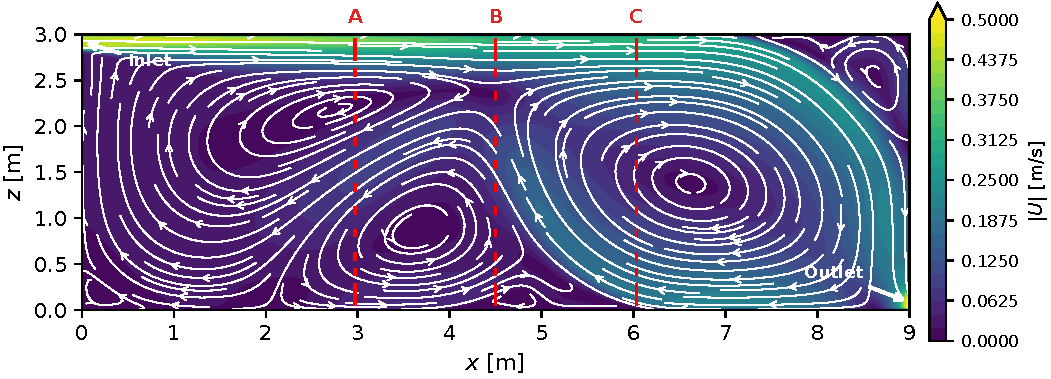
\includegraphics[width=\textwidth]{fig_method_validation_contour}
\caption{Solver validation against Nielsen et al. (1978) benchmark (9 m $\times$ 3 m, Re $\approx$ 5,000). Colour contours show velocity magnitude; white streamlines show the ceiling jet, recirculation zone, and corner vortex. Red markers (A, B, C) indicate the three LDA measurement stations compared in Table~\ref{tab:method-validation-nielsen}.}
\label{fig:method-validation-contour}
\end{figure*}

\begin{table}[htbp]
\centering
\caption{Solver validation: simpleFoam k-$\omega$ SST against Nielsen et al. (1978) LDA measurements at three vertical profiles (43,200 cells).}
\label{tab:method-validation-nielsen}
\begin{tabular}{llllll}
\toprule
Profile & $x/L$ & Points & Hit rate ($D$ = 0.25) & RMSE ($u/U_0$) & Pearson $R$ \\
\midrule
A & 0.33 & 16 & 0.125 & 0.250 & 0.788 \\
B & 0.50 & 16 & 0.188 & 0.227 & 0.806 \\
C & 0.67 & 16 & 0.000 & 0.332 & 0.932 \\
\textbf{Mean} & --- & \textbf{48} & \textbf{0.104} & \textbf{0.270} & \textbf{0.842} \\
\bottomrule
\end{tabular}
\end{table}


The Pearson correlation ($R$ = 0.842) confirms that the solver reproduces the qualitative velocity profile shape Fig.~\ref{fig:method-validation-contour}. The low hit rate ($q$ = 0.104) reflects quantitative magnitude differences in the low-speed recirculation region, consistent with known wall-function RANS limitations at moderate Reynolds numbers. A grid independence check (10,800 vs. 43,200 cells) showed negligible change in $R$ and hit rate. The solver accurately predicts flow topology but absolute velocity magnitudes carry approximately 27\% normalised RMSE uncertainty, which propagates into the velocity magnitude similarity component of the CFD agreement score. This validation is limited to a single 2D benchmark case; the 3D obstructed indoor flows in the benchmark are more complex, and the CFD agreement scores should be interpreted as relative comparisons between predicted and reference geometries rather than as absolute accuracy measures.

\subsection{Reference path and data-leakage prevention}
\label{sec:reference-path-and-data-leakage-prevention}


The reference CFD solution for each benchmark case is computed from the ground-truth scene JSON using the same meshing and solver pipeline described above Fig.~\ref{fig:method-eval-pathway}. The reference path does not involve any VLM invocation: the ground-truth scene is generated by the rule-based benchmark generator and is never presented to Gemini. The 2D input images are rendered from the 3D ground-truth scene, but these renderings are used only as inputs to the VLM and do not participate in the reference CFD computation. This separation ensures that the evaluation is free from circular reasoning or data leakage.

\begin{figure*}[htbp]
\centering
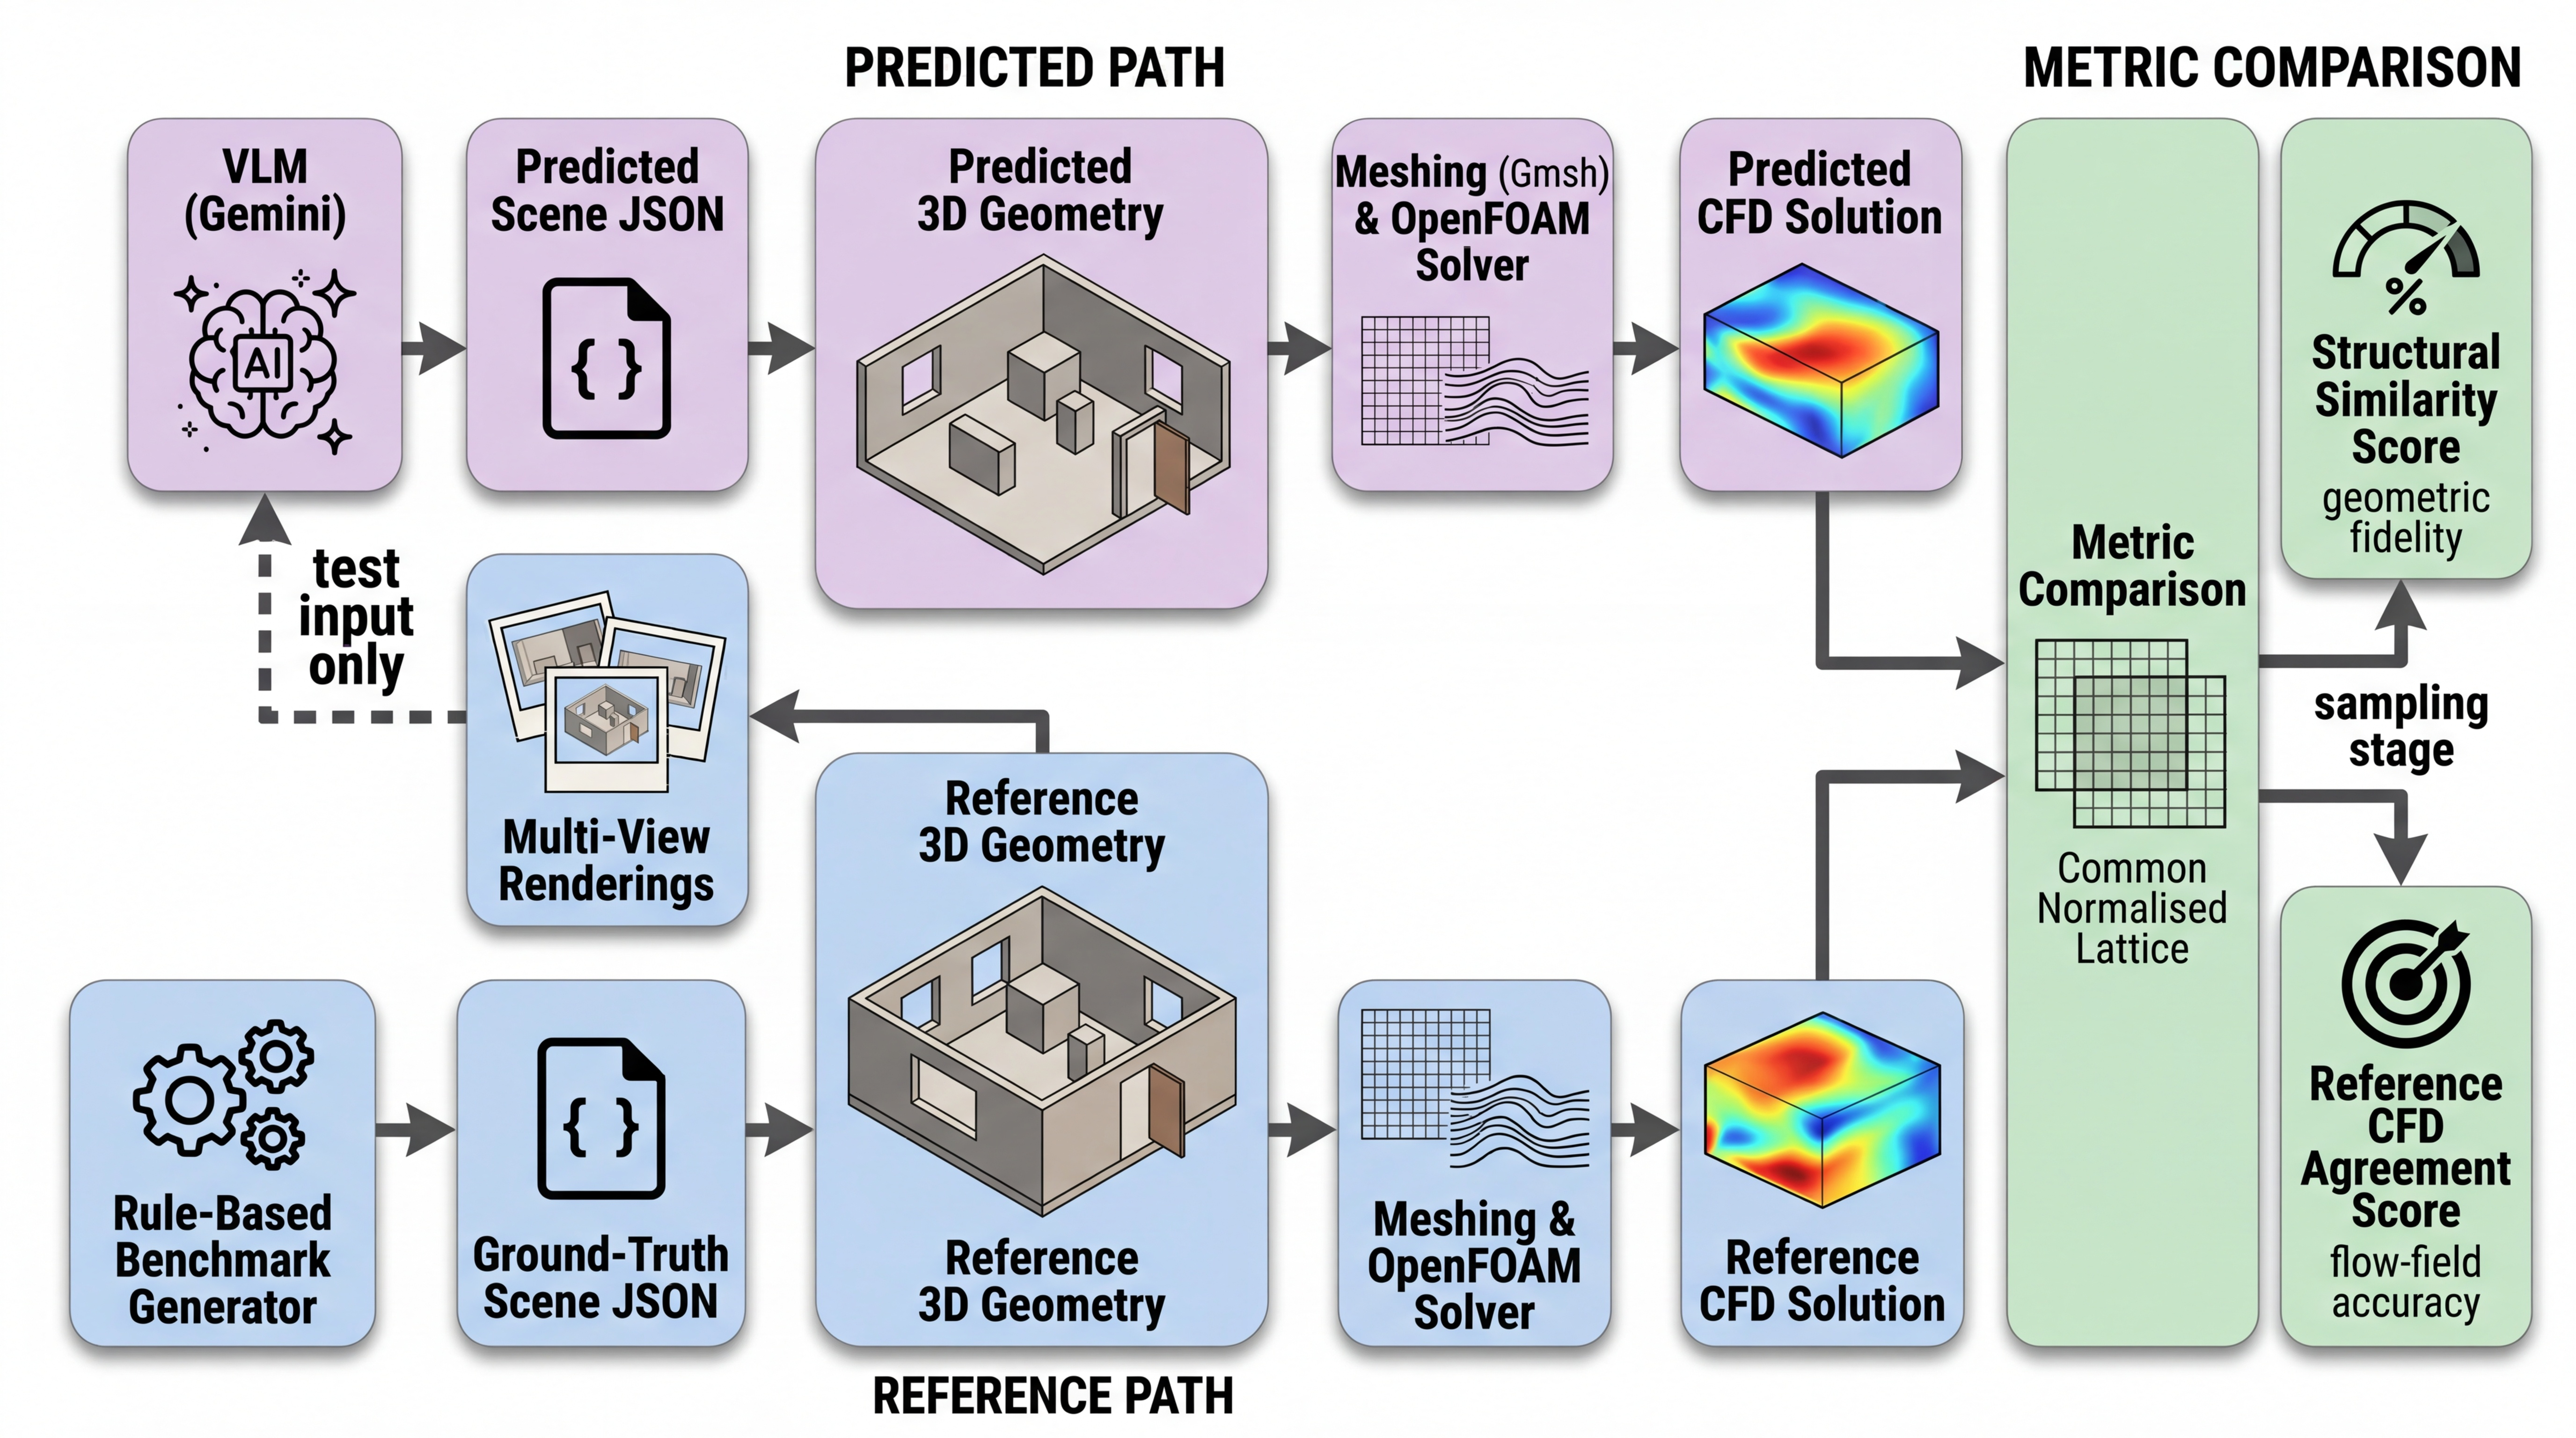
\includegraphics[width=\textwidth]{fig_method_eval_pathway}
\caption{Evaluation pathway. The predicted path (top) processes the 2D input through VLM, scale calibration, and CFD; the reference path (bottom) uses the rule-based ground-truth scene directly. Both paths converge at the metric comparison stage.}
\label{fig:method-eval-pathway}
\end{figure*}


\section{Benchmark Dataset}
\label{sec:benchmark-dataset}


\subsection{Geometry design}
\label{sec:geometry-design}


The benchmark dataset comprises 20 indoor geometries organised into a 2 x 2 complexity matrix along two independent axes: room topology (rectangular versus composite L-shaped) and obstacle density (simple versus dense). The four resulting categories are designated A1 through A4 Fig.~\ref{fig:bench-design}. Category A1 contains simple rectangular rooms with zero or one obstacle, serving as a positive control where the framework is expected to perform well. Category A2 adds two to three obstacles to the rectangular room, introducing clutter without topological complexity. Category A3 replaces the rectangular room with an L-shaped composite geometry formed by the Boolean union of two axis-aligned blocks, while keeping obstacle density low. Category A4 combines the composite topology with dense obstacle placement, representing the most challenging condition. Each category contains five independently generated cases, yielding 20 geometries in total. Fig.~\ref{fig:bench-cfd-showcase} shows a representative case from each category with its reference CFD velocity field, illustrating the range of geometric complexity and the corresponding flow patterns.

\begin{figure*}[htbp]
\centering
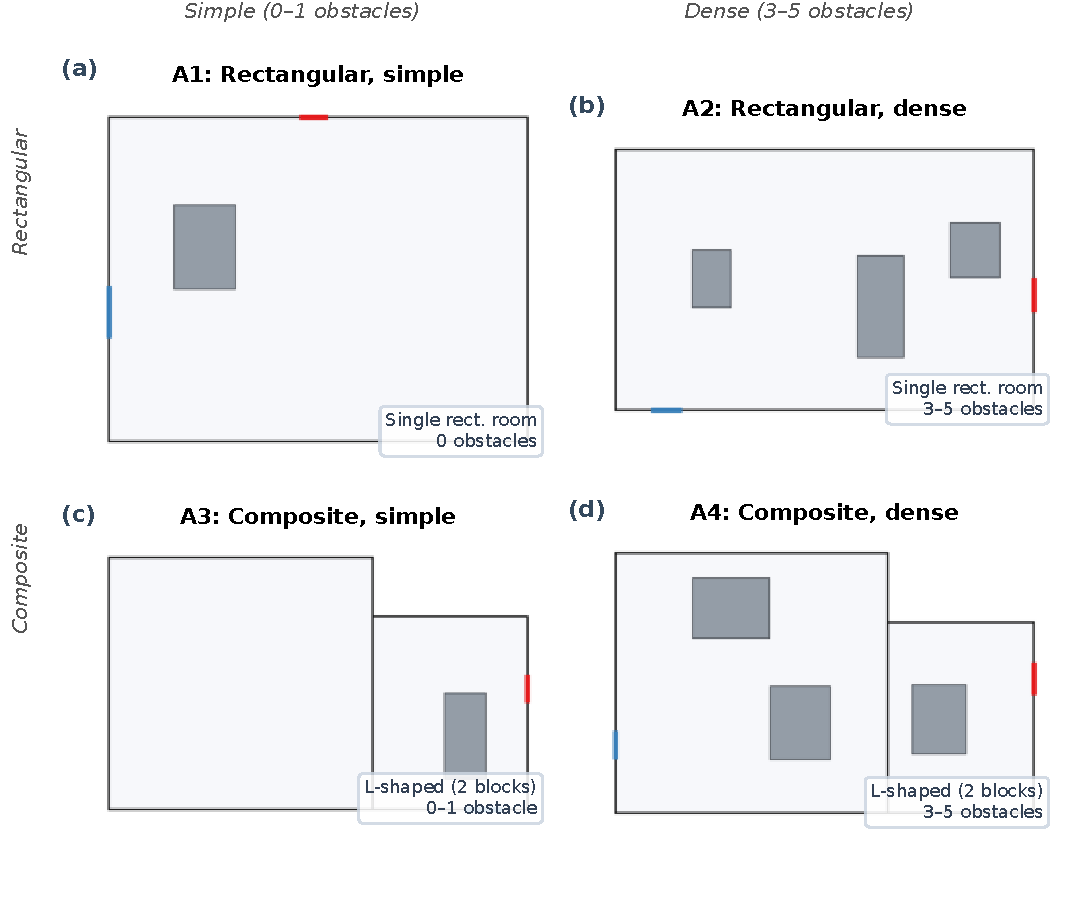
\includegraphics[width=\textwidth]{fig_bench_design}
\caption{Benchmark dataset design. The 20 geometries are organised into a 2 $\times$ 2 matrix of room topology (rectangular vs. composite L-shaped) and obstacle density (simple vs. dense), yielding categories A1--A4; the summary table reports per-category evaluation statistics.}
\label{fig:bench-design}
\end{figure*}

\begin{figure*}[htbp]
\centering
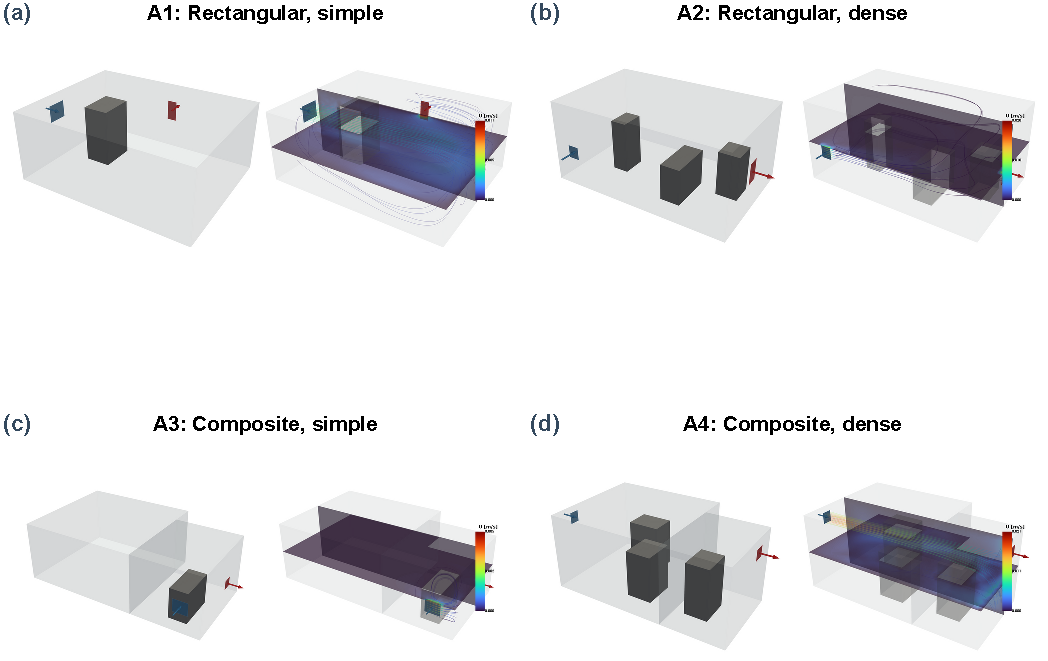
\includegraphics[width=\textwidth]{fig_bench_cfd_showcase}
\caption{Representative reference cases from each complexity category: 3D geometry (left) and steady-state CFD velocity field with streamlines (right). (a) A1, (b) A2, (c) A3, (d) A4.}
\label{fig:bench-cfd-showcase}
\end{figure*}

All geometries are generated by a deterministic rule-based generator with fixed random seeds to ensure reproducibility. Room dimensions are sampled uniformly within realistic ranges (3 to 8 m in length, 3 to 6 m in width, 2.4 to 3.5 m in height). Obstacles are placed with a minimum wall clearance of 0.4 m and a minimum inter-obstacle clearance sufficient to avoid degenerate mesh cells. Each room has exactly one inlet and one outlet, placed on different walls. Opening sizes are sampled from a range of 0.3 to 1.0 m in each dimension, consistent with typical indoor ventilation diffuser dimensions.

\subsection{Multi-view rendering protocol}
\label{sec:multi-view-rendering-protocol}


Each of the 20 benchmark geometries is rendered into five distinct 2D input views Fig.~\ref{fig:bench-multiview}: perspective, bird's-eye, floor plan, wireframe, and section. The perspective view provides a natural photographic viewpoint with depth cues and foreshortening. The bird's-eye view offers a top-down oblique angle that reveals the overall layout. The floor-plan view is an orthographic top-down projection that preserves planimetric proportions but eliminates height information. The wireframe view renders the geometry as line edges without surface shading. The section view shows a vertical cut through the room, revealing the cross-sectional profile but obscuring features outside the cutting plane. Rendering all five views from each geometry yields 100 input images in total, enabling a controlled analysis of how input view type affects downstream prediction quality while holding the underlying geometry constant.

\begin{figure*}[htbp]
\centering
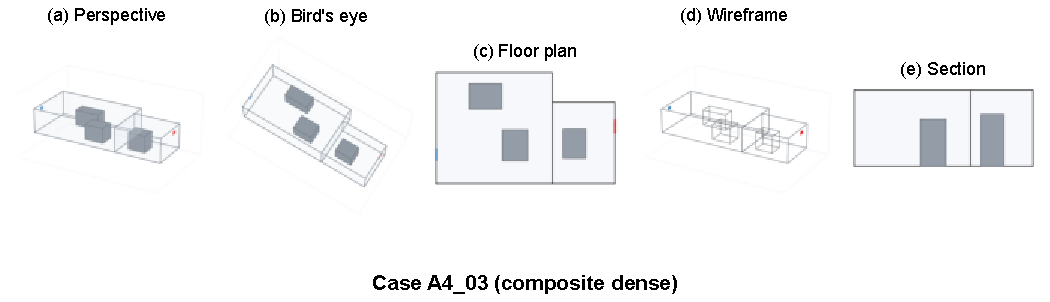
\includegraphics[width=\textwidth]{fig_bench_multiview}
\caption{Multi-view rendering protocol. The same geometry (A4-03) rendered into five input views: (a) perspective, (b) bird's-eye, (c) floor plan, (d) wireframe, and (e) section, illustrating the variation in information content.}
\label{fig:bench-multiview}
\end{figure*}

\subsection{Scale calibration}
\label{sec:scale-calibration}


The VLM does not have access to absolute dimensional references in the input image, and its predicted scene dimensions therefore exhibit a systematic scale error. To correct this, a single-factor post-hoc scaling is applied: the longest horizontal span in the predicted geometry is identified, and the ratio between this span and the corresponding span in the reference geometry is used as a uniform scale factor applied to all coordinates. After calibration, the mean relative error in the scaled dimension (Lx) drops to 0.4\%, while the remaining dimensions retain relative errors of approximately 22\% (Ly) and 20\% (Lz). This residual anisotropy reflects the VLM's tendency to estimate the dominant room dimension more accurately than secondary dimensions, and it is a known limitation of single-factor calibration.


\section{Results}
\label{sec:results}


\subsection{Aggregate performance}
\label{sec:aggregate-performance}


To contextualise the framework's performance, a naive geometric baseline is evaluated alongside the scale-calibrated pipeline. The baseline predicts a fixed 5 m $\times$ 4 m $\times$ 3 m rectangular room with no obstacles and one inlet-outlet pair on opposite walls for every case. Table~\ref{tab:result-baseline-comparison} compares the two conditions.

\begin{table}[htbp]
\centering
\caption{Structural score comparison: naive baseline versus scale-calibrated VLM pipeline (n = 100).}
\label{tab:result-baseline-comparison}
\begin{tabular}{llll}
\toprule
Condition & Structural score & Room-kind match & Opening-wall match \\
\midrule
Naive geometric default & 0.621 & 50\% & 80\% \\
VLM, scale-calibrated & 0.781 & 95\% & 70\% \\
\bottomrule
\end{tabular}
\end{table}


Note: the naive baseline achieves a higher opening-wall match rate (80\%) than the VLM (70\%) because the fixed west-inlet/east-outlet assignment happens to match many reference cases by chance, not because of superior spatial reasoning.

The scale-calibrated framework achieves a mean structural score of 0.781 (+25.8\% relative over the naive baseline). The baseline's non-trivial score of 0.621 reflects that the structural metric rewards correct opening-type classification even when dimensions and obstacles are wrong. The VLM achieves a substantially higher room-kind match rate (95\% vs. 50\%), confirming reliable rectangular/composite topology discrimination that a fixed-geometry baseline cannot perform.

To further clarify the contribution of each evaluation component, Table~\ref{tab:result-component-breakdown} decomposes the structural score into its four constituents for both the naive baseline and the scale-calibrated pipeline.

\begin{table}[htbp]
\centering
\caption{Component-level breakdown of the structural score.}
\label{tab:result-component-breakdown}
\begin{tabular}{lll}
\toprule
Component & Naive & Scale-calibrated \\
\midrule
Room block F1 (IoU $\geq$ 0.2) & 0.833 & 0.988 \\
Obstacle F1 (IoU $\geq$ 0.1) & 0.150 & 0.400 \\
Opening type F1 & 1.000 & 1.000 \\
Opening wall match ratio & 0.500 & 0.737 \\
\textbf{Overall structural score} & \textbf{0.621} & \textbf{0.781} \\
\bottomrule
\end{tabular}
\end{table}


Opening type F1 is trivially 1.0 for both conditions because the benchmark design specifies exactly one inlet and one outlet per case, guaranteeing a perfect match regardless of method. This component contributes a fixed 0.25 to the overall structural score; the remaining three components carry the discriminative power. Opening wall match ratio improves from 0.500 (naive, chance alignment) to 0.737 (VLM), confirming genuine spatial reasoning about which walls carry openings. Room block F1 is near-perfect for the VLM (0.988) after scale calibration, while obstacle F1 is the weakest component (0.400), accounting for most of the gap between current performance and a perfect score. The naive baseline's obstacle F1 of 0.150 is non-zero only because a small number of reference cases have zero obstacles.

The mean reference CFD agreement score is 0.477. Component decomposition Fig.~\ref{fig:result-cfd-component-breakdown} shows overlap ratio (0.888) and velocity direction similarity (0.634) are moderate to high, while velocity magnitude similarity (0.117) is low across all views and pressure similarity (0.269) is intermediate. These values indicate qualitatively correct flow patterns but quantitatively different velocity magnitudes. CFD baselines are not computed for the naive default condition, as that baseline exists only to contextualise the structural score.

\begin{figure*}[htbp]
\centering
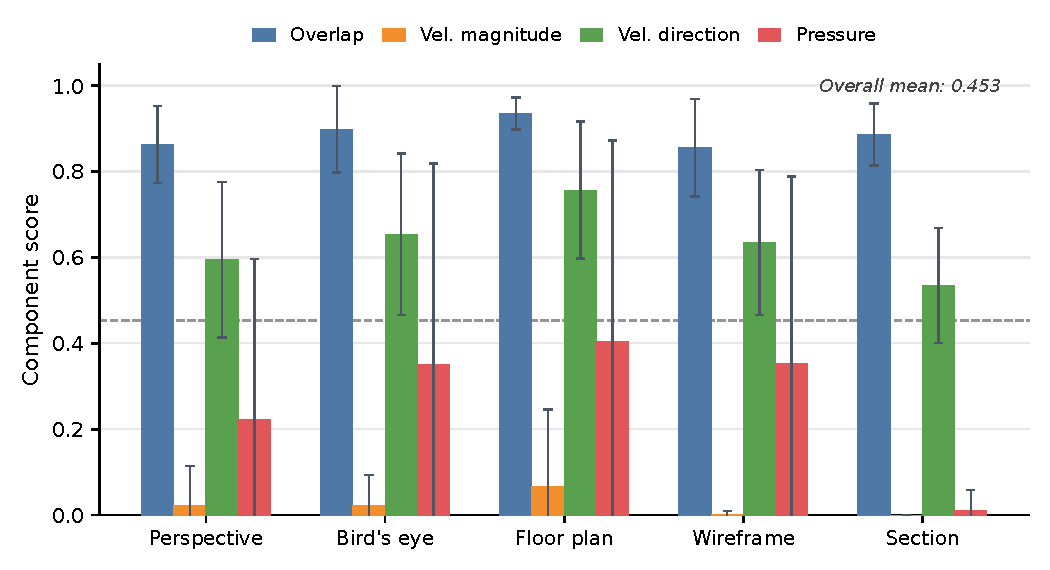
\includegraphics[width=\textwidth]{fig_result_cfd_component_breakdown}
\caption{CFD agreement score decomposed into four components (overlap ratio, velocity magnitude similarity, direction similarity, pressure similarity) by view type, with standard-deviation error bars. Velocity magnitude is near zero across all views, driving the low overall score despite moderate overlap and directional agreement.}
\label{fig:result-cfd-component-breakdown}
\end{figure*}

For reference, the COST 732 standard metrics averaged across all 97 cases yield a velocity magnitude hit rate of q = 0.09, FAC2 = 0.28, and a Pearson correlation of R = 0.44, confirming the limited quantitative velocity agreement identified by the agreement score decomposition.

\begin{table}[htbp]
\centering
\caption{Detailed evaluation results for the scale-calibrated pipeline (n = 97 valid cases out of 100; three cases excluded due to solver divergence failures).}
\label{tab:result-detailed-metrics}
\begin{tabular}{ll}
\toprule
Metric & Value \\
\midrule
Mean structural score & 0.781 $\pm$ 0.150 \\
Mean CFD agreement score & 0.477 $\pm$ 0.158 \\
Room-kind match rate & 95\% \\
Opening-wall match rate & 70\% \\
Mean Lx relative error & 0.4\% \\
Mean Ly relative error & 21.9\% \\
Mean Lz relative error & 19.8\% \\
Mean volume relative error & 36.6\% \\
Solver divergence failures & 3 / 100 \\
\bottomrule
\end{tabular}
\end{table}


Three cases (bench\_a3\_04/perspective, bench\_a4\_02/perspective, bench\_a4\_02/wireframe) failed to converge due to non-physical predicted geometries. These are excluded from CFD score aggregation but counted in the structural and match statistics. For transparency, the unconditional scores (assigning 0.0 to the 3 failed cases) are: structural 0.758, CFD agreement 0.463. The conditional scores reported above (n = 97) are used throughout the paper unless noted otherwise.

\subsection{Effect of input view type}
\label{sec:effect-of-input-view-type}


The input view type has a pronounced effect on performance Fig.~\ref{fig:result-view-aggregate}. The floor-plan view achieves the highest scores (structural 0.884 $\pm$ 0.110, CFD 0.572 $\pm$ 0.185), consistent with its orthographic top-down projection preserving planimetric information. Rankings for the remaining views are: bird's-eye (0.800, 0.495), perspective (0.782, 0.443), wireframe (0.760, 0.476), and section (0.679, 0.396).

\begin{figure*}[htbp]
\centering
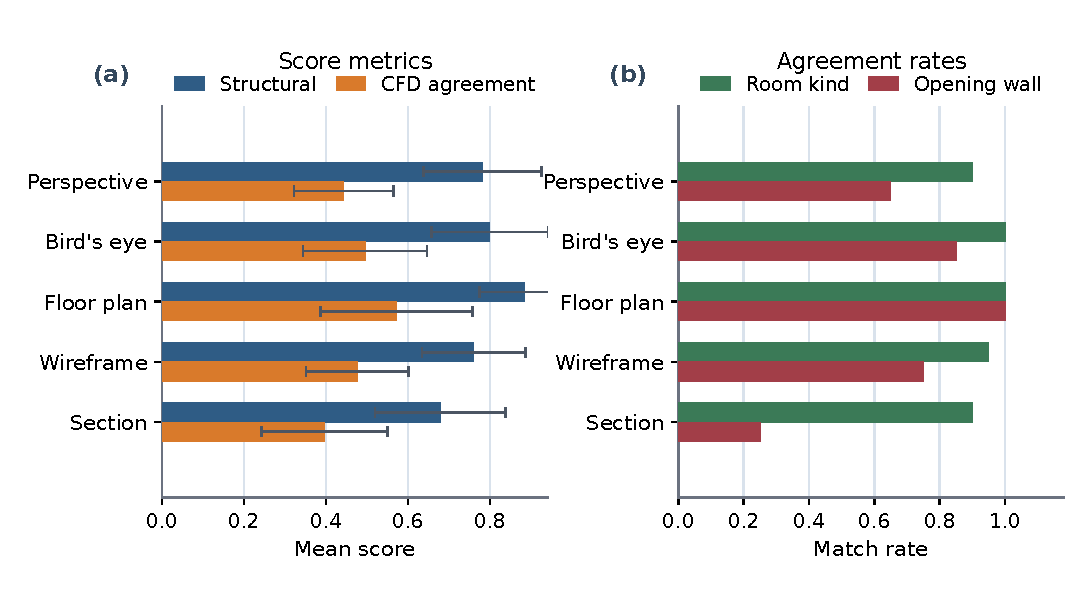
\includegraphics[width=\textwidth]{fig_result_view_aggregate}
\caption{Aggregate performance by input view type. (a) Mean structural and CFD scores. (b) Room-kind and opening-wall match rates. Floor plan achieves the highest performance across all metrics.}
\label{fig:result-view-aggregate}
\end{figure*}

Opening-wall match rate shows the most dramatic view dependence: floor plan 100\%, bird's-eye 85\%, wireframe 75\%, perspective 65\%, and section only 25\%. The section view's poor performance arises because a vertical cutting plane typically intersects only one or two walls, leaving remaining openings invisible to the VLM. Room-kind match rate is more robust, ranging from 90\% (perspective and section) to 100\% (bird's-eye and floor plan), as topology identification depends more on the overall room silhouette than on fine-grained wall visibility.

\subsection{Effect of geometric complexity}
\label{sec:effect-of-geometric-complexity}


Performance varies across complexity categories Fig.~\ref{fig:result-category-aggregate}. A1 (simple rectangular) achieves the highest scores (structural 0.845, CFD 0.519). A2 (rectangular dense) yields the lowest structural score (0.707) despite simpler room topology, because higher obstacle density increases placement errors. A3 and A4 (composite) achieve structural scores of 0.783 and 0.791, showing that composite topology alone does not severely degrade structural prediction; CFD scores are 0.498 (A2), 0.480 (A3), and 0.407 (A4).

\begin{figure*}[htbp]
\centering
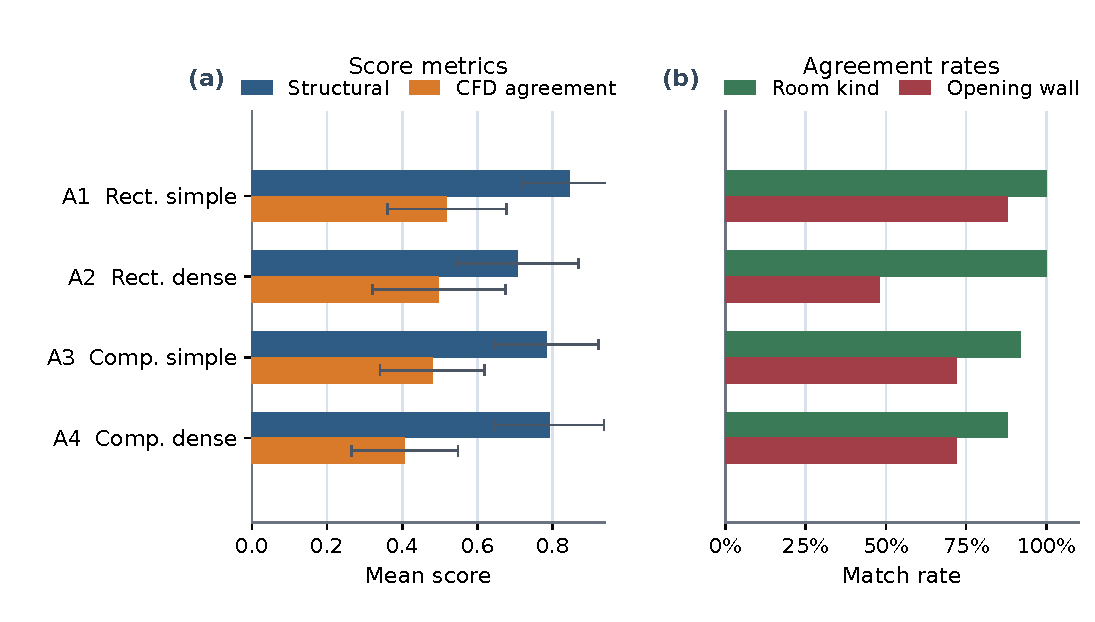
\includegraphics[width=\textwidth]{fig_result_category_aggregate}
\caption{Aggregate performance by benchmark category. (a) Mean structural and CFD scores. (b) Room-kind and opening-wall match rates.}
\label{fig:result-category-aggregate}
\end{figure*}

Opening-wall match rates differ: A1 88\%, A3 and A4 each 72\%, A2 only 48\%. The low A2 rate reflects the geometric equivalence of all four walls in a rectangular room, leaving the VLM without topological cues. In composite rooms, the L-shaped topology provides a spatial anchor that improves opening-wall assignment.

\subsection{Solver robustness}
\label{sec:solver-robustness}


Of the 100 cases, 97 produce a converged solution and 3 fail due to solver divergence from non-physical predicted geometries. Of the 97 converged cases, the majority converge under the nominal solver configuration; the remainder require escalation through the robustness pathway Fig.~\ref{fig:result-robustness}. Three cases fail entirely and are excluded from CFD score aggregation. The escalation rate is highest for the section view and the floor-plan view, the latter driven by cases where the accurate geometry produces complex internal flow structures that challenge the turbulence model at the nominal mesh resolution.

\begin{figure*}[htbp]
\centering
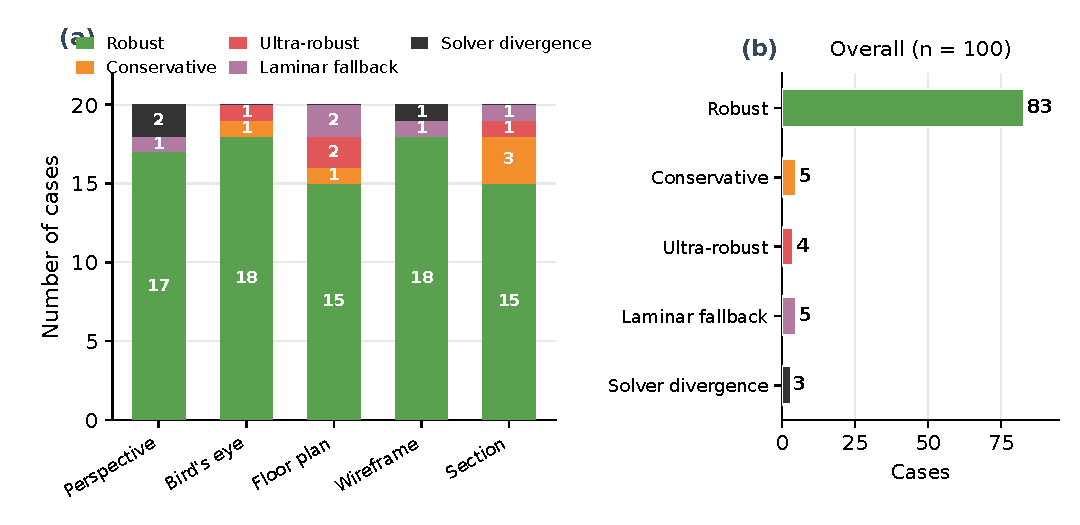
\includegraphics[width=\textwidth]{fig_result_robustness}
\caption{Robustness and convergence summary.}
\label{fig:result-robustness}
\end{figure*}

\subsection{VLM output repeatability}
\label{sec:vlm-output-repeatability}


Because the VLM operates with a sampling temperature of 0.2, its output is stochastic rather than deterministic. To characterise this variation, three representative cases (bench\_a1\_01, bench\_a3\_03, bench\_a4\_03) were each processed three times through the floor-plan pipeline. Table~\ref{tab:result-vlm-repeatability} reports the structural scores across runs.

\begin{table}[htbp]
\centering
\caption{VLM repeatability: structural scores across 3 independent runs per case (floor-plan view).}
\label{tab:result-vlm-repeatability}
\begin{tabular}{lllll}
\toprule
Case & Run 1 & Run 2 & Run 3 & Mean $\pm$ SD \\
\midrule
A1-01 (simple) & 0.875 & 0.875 & 0.875 & 0.875 $\pm$ 0.000 \\
A3-03 (composite) & 1.000 & 0.875 & 0.875 & 0.917 $\pm$ 0.059 \\
A4-03 (dense) & 0.917 & 1.000 & 1.000 & 0.972 $\pm$ 0.039 \\
\bottomrule
\end{tabular}
\end{table}


The mean standard deviation is 0.033. Room topology (room block F1 = 1.0) and opening-wall assignment (wall match ratio = 1.0) are perfectly consistent across all runs; variation arises solely from obstacle matching. Raw room dimensions vary substantially between runs (e.g., scale factors of 0.54, 1.08, and 0.86 for the same case), confirming that post-hoc scale calibration is essential. The small sample size (9 observations) limits statistical power; a larger study is needed to fully characterise VLM stochastic variation.


\section{Discussion}
\label{sec:discussion}


\subsection{Failure mode I: composite-room collapse under section view}
\label{sec:failure-mode-i-composite-room-collapse-under-section-view}


When a section cutting plane passes through only one block of an L-shaped room, the VLM infers a rectangular room and discards the second block entirely Fig.~\ref{fig:discuss-section-collapse}. This collapse eliminates recirculation zones present in the reference solution and degrades both structural and CFD scores. The failure is inherent to the section view's limited information content: a vertical section through an L-shaped room is geometrically indistinguishable from a rectangular section unless the plane intersects the block junction. Section views should therefore be avoided for suspected non-rectangular topologies, or supplemented with a second view.

\begin{figure*}[htbp]
\centering
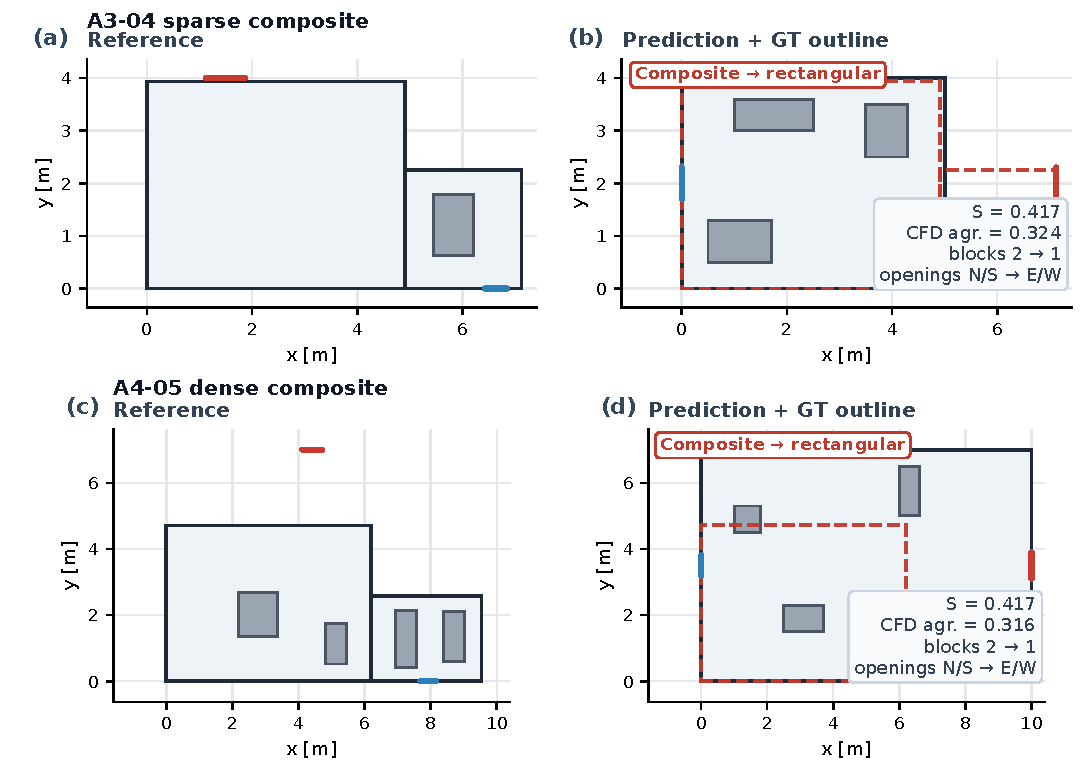
\includegraphics[width=\textwidth]{fig_discuss_section_collapse}
\caption{Composite-room collapse under section view. Cases A3-04 and A4-05 are shown with reference geometry (left) and VLM prediction with ground-truth overlay (right); the VLM collapses the L-shaped room to a single rectangular block in both cases.}
\label{fig:discuss-section-collapse}
\end{figure*}

\subsection{Failure mode II: obstacle hallucination with limited CFD penalty}
\label{sec:failure-mode-ii-obstacle-hallucination-with-limited-cfd-penalty}


The VLM frequently predicts obstacles absent from the reference, particularly in wireframe and section views where sparse visual cues are misinterpreted as internal structures Fig.~\ref{fig:discuss-obstacle-hallucination}. In two representative A3 wireframe cases, obstacle counts inflate from 0 to 3 and from 1 to 3, yet CFD agreement scores remain 0.380 and 0.529, with opening assignments preserved. Hallucinated obstacles tend to be small relative to room volume and sit away from the main flow path, so they disturb the local velocity field but leave bulk ventilation patterns intact. Obstacle prediction errors are therefore tolerable when the primary interest is bulk airflow rather than near-furniture velocity detail.

\begin{figure*}[htbp]
\centering
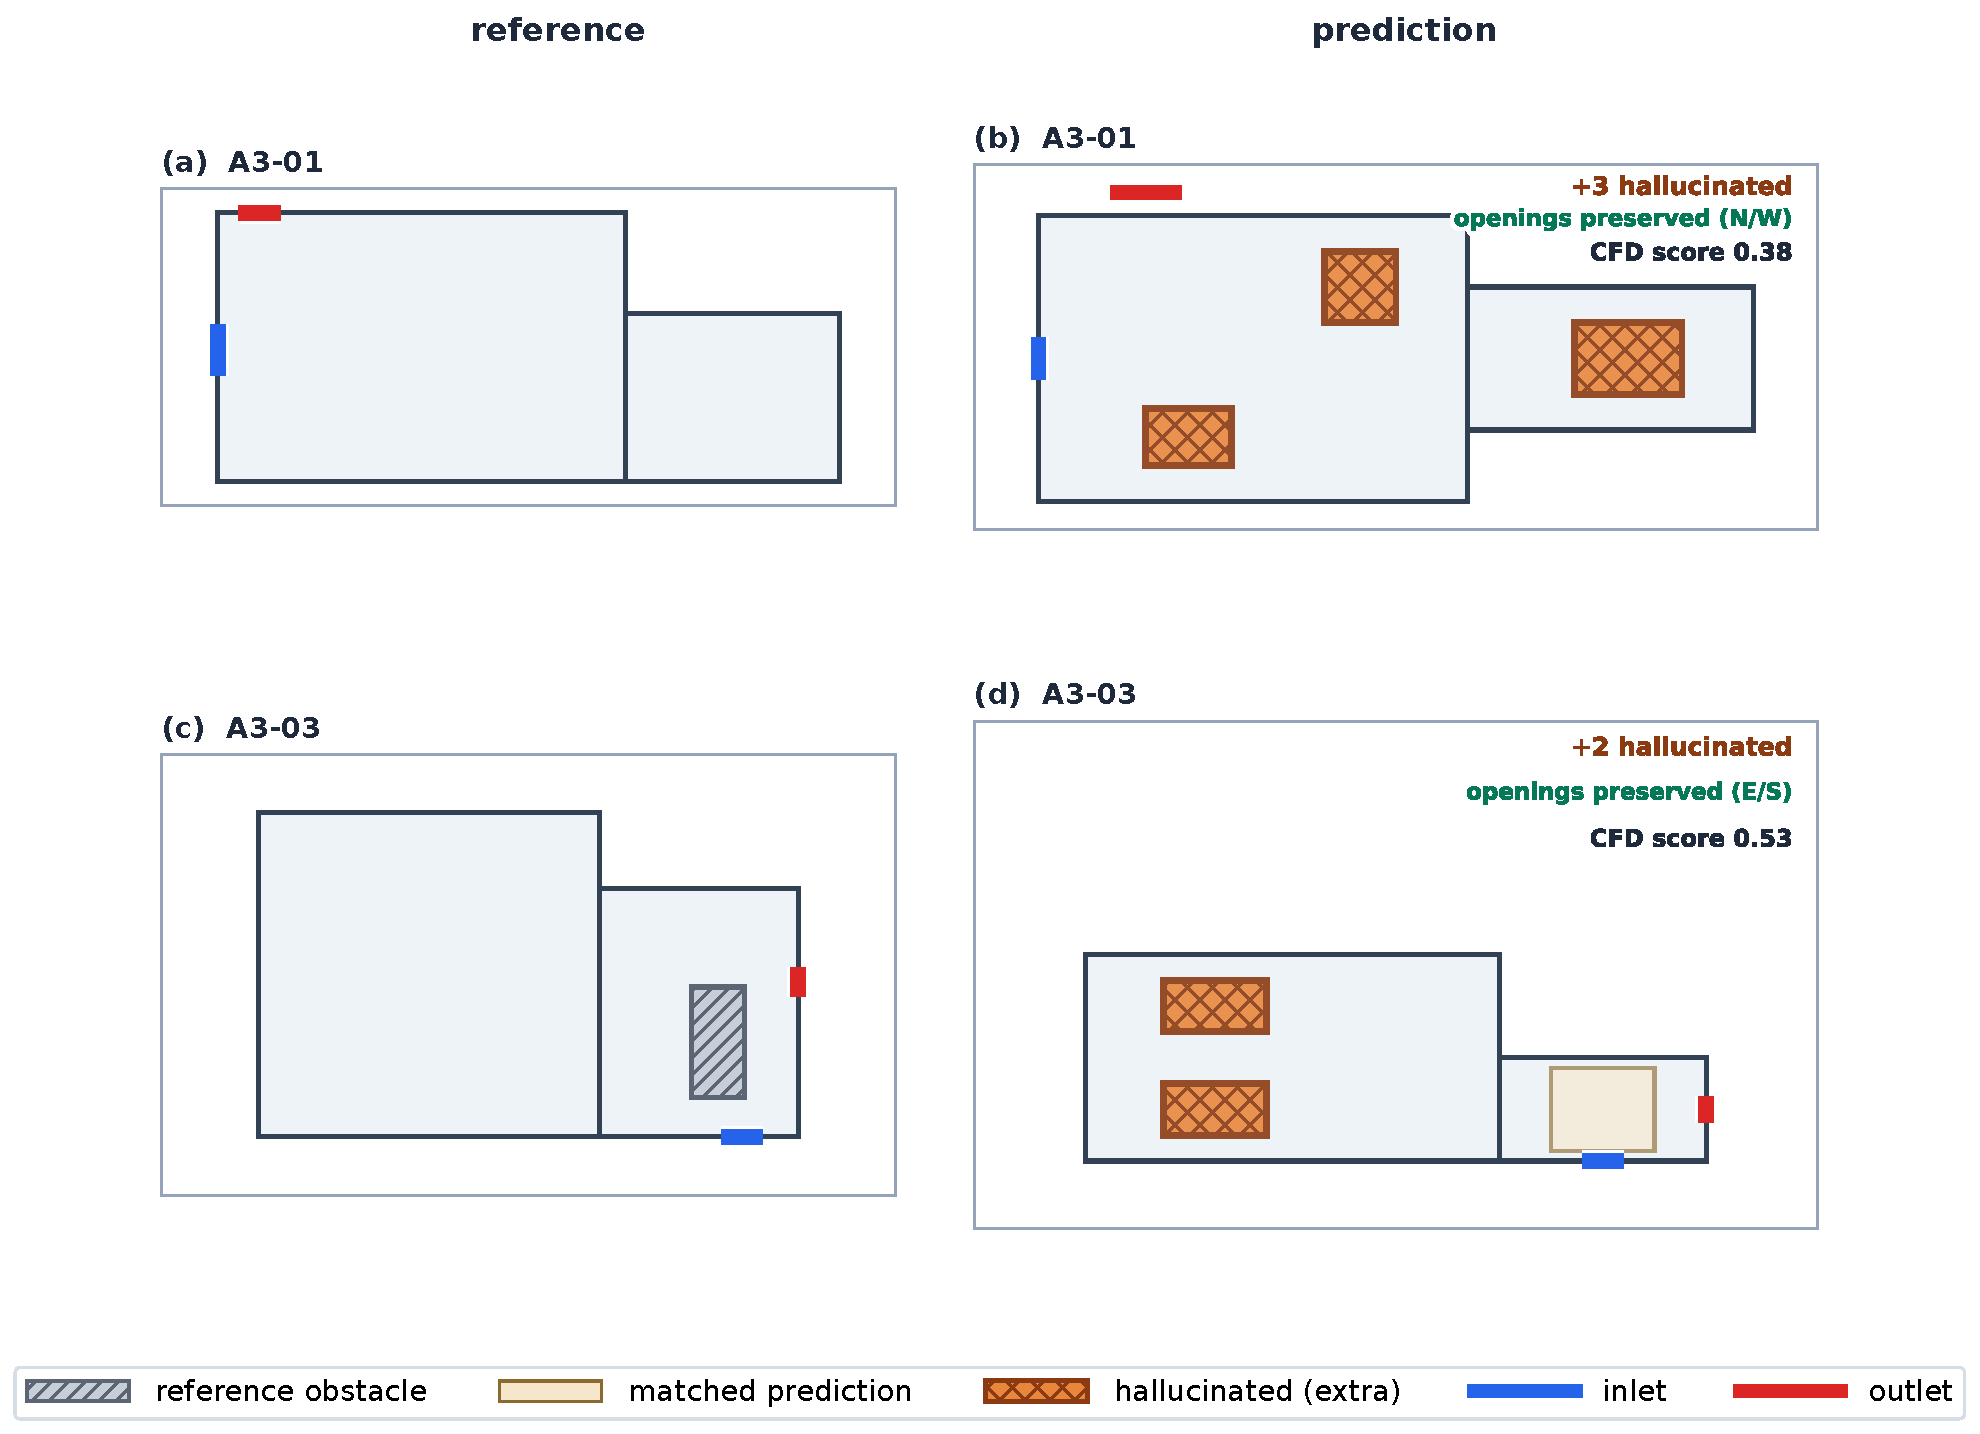
\includegraphics[width=\textwidth]{fig_discuss_obstacle_hallucination}
\caption{Obstacle hallucination with limited CFD penalty. Two A3 wireframe cases show obstacle count inflation (0 $\rightarrow$ 3 and 1 $\rightarrow$ 3); hallucinated obstacles (orange cross-hatch) are distinguished from matched predictions (tan). Opening topology is preserved and CFD scores remain 0.380 and 0.529.}
\label{fig:discuss-obstacle-hallucination}
\end{figure*}

\subsection{Failure mode III: structure-versus-fidelity gap in dense composites}
\label{sec:failure-mode-iii-structure-versus-fidelity-gap-in-dense-composites}


Structural and CFD scores are only weakly correlated across all 97 valid cases Fig.~\ref{fig:discuss-scatter-struct-cfd}. The decoupling is most pronounced in A4: case A4-02 achieves a structural score of 0.813 yet a CFD score of only 0.346; case A4-04 scores 0.917 structurally yet 0.302 in CFD Fig.~\ref{fig:discuss-structure-cfd-gap}. In dense obstacle configurations, the flow field is sensitive to small geometric perturbations: misalignments of a few centimetres, even within the IoU matching threshold, can redirect jets, create or eliminate recirculation zones, and shift stagnation points. Bounding-box structural matching alone does not guarantee CFD fidelity in these cases.

\begin{figure*}[htbp]
\centering
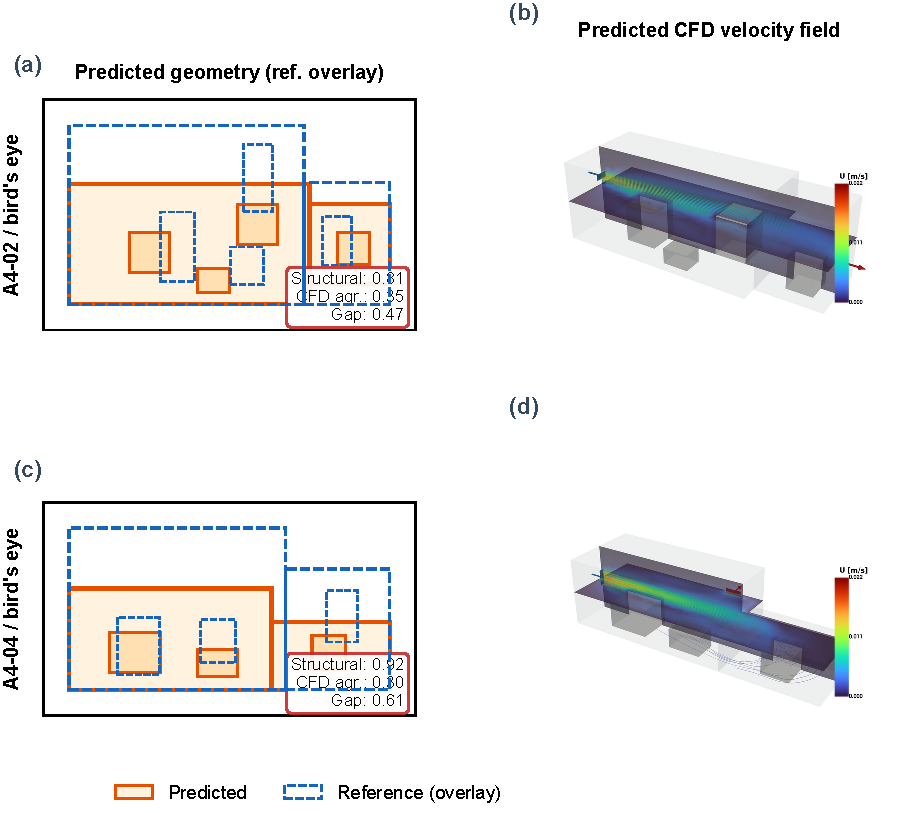
\includegraphics[width=\textwidth]{fig_discuss_structure_cfd_gap}
\caption{Structure-versus-fidelity gap in dense composites. Two A4 cases with high structural scores (0.938 and 1.000) achieve low CFD scores (0.409 and 0.458); left panels show geometry overlap, right panels compare flow fields.}
\label{fig:discuss-structure-cfd-gap}
\end{figure*}

\begin{figure*}[htbp]
\centering
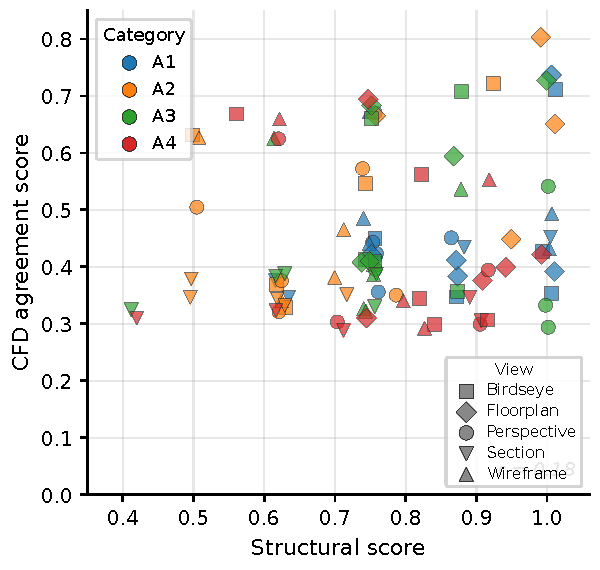
\includegraphics[width=\textwidth]{fig_discuss_scatter_struct_cfd}
\caption{Structural score versus CFD agreement score for all 97 valid cases.}
\label{fig:discuss-scatter-struct-cfd}
\end{figure*}

\subsection{Scale calibration and its limitations}
\label{sec:scale-calibration-and-its-limitations}


The single-factor scaling requires one user-provided dimension, the minimum input needed for physically meaningful CFD from a monocular image. This is an intentional design choice: absolute scale cannot be inferred from a single image regardless of the VLM's capability, and omitting it would produce dimensionally arbitrary results unsuitable for engineering use. In the benchmark, this dimension is taken from the ground-truth geometry; in practice, a single tape measurement or a dimension annotation on the drawing suffices.

The calibration reduces the mean Lx error to 0.4\% but leaves the secondary dimensions (Ly, Lz) with relative errors of approximately 20\%. This anisotropic residual error distorts the room volume (affecting bulk velocity magnitude for a given inlet flow rate) and alters the aspect ratio (shifting reattachment points and recirculation zones). A multi-factor calibration correcting each dimension independently would reduce these errors but would require multiple measurements, adding user burden. The single-factor approach balances accuracy against practical simplicity.

\subsection{Reference solver preset matching}
\label{sec:reference-solver-preset-matching}


To ensure fair flow-field comparison, the reference CFD solution for each benchmark case was computed using the same solver preset, and therefore the same inlet velocity boundary condition, as the corresponding predicted case. This preset matching eliminates systematic velocity scale discrepancies that would arise when different cases require different levels of solver stabilisation to achieve convergence at the 0.18 m mesh resolution.

\subsection{Computational cost}
\label{sec:computational-cost}


The end-to-end pipeline time per case is approximately 3 to 8 minutes on a single workstation, depending on the mesh resolution and solver convergence behaviour. The VLM API call (Gemini 3.1 Pro) typically returns within 10 to 30 seconds. Mesh generation with Gmsh takes 5 to 15 seconds at the nominal 0.18 m cell size. The dominant cost is the steady-state CFD solve, which ranges from 1 to 6 minutes depending on the case complexity and whether solver escalation is triggered. Manual geometry preparation for a comparable indoor space typically takes hours of CAD work; the automated pipeline replaces this with minutes.

\subsection{Practical considerations and limitations}
\label{sec:practical-considerations-and-limitations}


The current study has several limitations. First, all results reported in this paper use a mesh cell size of 0.18 m for both reference and predicted cases. A grid independence study was conducted on three representative cases at cell sizes of 0.35, 0.25, 0.18, and 0.10 m. Table~\ref{tab:discuss-grid-independence} shows the reference CFD agreement score evaluated at each reference resolution against the same predicted solution.

\begin{table}[htbp]
\centering
\caption{Grid independence check: reference CFD agreement score evaluated against reference solutions at four mesh resolutions, spanning a 34$\times$ range in cell count. All predicted solutions use a cell size of 0.18 m.}
\label{tab:discuss-grid-independence}
\begin{tabular}{lllllll}
\toprule
Case & Cells (0.18 m) & Ref. 0.35 m & Ref. 0.25 m & Ref. 0.18 m & Ref. 0.10 m & $\Delta$ max \\
\midrule
A1-01 & ~37,000 & 0.389 & 0.568 & 0.579 & 0.625 & 0.236 \\
A3-03 & ~62,000 & 0.739 & 0.726 & 0.641 & 0.616 & 0.123 \\
A4-03 & ~55,000 & 0.576 & 0.553 & 0.558 & 0.598 & 0.045 \\
\bottomrule
\end{tabular}
\end{table}


At 0.35 m, mean velocities are underpredicted by up to 50\% for simple geometries, confirming that resolution is inadequate for quantitative comparison. From 0.18 m onward, key quantities change less than 5\% upon further refinement to 0.10 m; 0.18 m was therefore selected as the operational mesh size (3--8 min per case vs. 30+ min at 0.10 m). The non-monotonic trend for A3-03 (score decreasing from 0.739 to 0.616 with finer reference mesh) reflects that a more refined reference exposes geometric discrepancies masked at coarser resolution. Relative case rankings are preserved across all resolutions.

Second, the benchmark uses only axis-aligned rectangular and L-shaped rooms; curved walls, sloped ceilings, and multi-storey configurations are not evaluated. Third, steady-state isothermal RANS may not capture transient flow features, complex turbulence in densely obstructed rooms, or buoyancy-driven stratification important in energy audit scenarios; extension to conjugate heat transfer or buoyant flow models is left as future work. Fourth, the intersection-domain comparison may under-represent errors where predicted rooms extend beyond or fall short of the reference domain, and single-factor scale calibration requires one known reference dimension that may be unavailable in fully unsupervised deployment. Fifth, all results use a single VLM (Gemini 3.1 Pro, preview, accessed March 2026); the framework architecture is VLM-agnostic, but the reported scores are specific to this model version, and a multi-model comparison is left as future work.


\section{Application to Architectural Floor Plans}
\label{sec:application-to-architectural-floor-plans}


As a qualitative demonstration of the framework on non-synthetic inputs, two architectural floor plan images were prepared and processed through the full pipeline. No ground-truth reference CFD is available for these cases; the results are assessed only for geometric plausibility and solver convergence, not for quantitative accuracy. Both cases use the floor-plan view, which achieved the highest performance in the benchmark evaluation (structural score 0.884, opening-wall match 100\%).

The first case is a simple rectangular office of 6.0 m $\times$ 4.0 m (Fig.~\ref{fig:demo-floorplan-application}a). The floor plan includes hatched walls, a door with arc symbol on the south wall, a window on the north wall, and three furniture items (desk, chair, shelf). Dimension annotations on the drawing provide the scale reference. The VLM correctly identifies the rectangular room topology with dimensions 6.0 $\times$ 4.0 $\times$ 2.7 m, places three obstacles corresponding to the furniture items, and assigns the door as inlet (south wall) and the window as outlet (north wall). The resulting CFD simulation converges under the robust solver preset at 0.18 m mesh resolution, producing a physically plausible flow field with a jet from the south-wall inlet traversing the room toward the north-wall outlet (Fig.~\ref{fig:demo-floorplan-application}b).

\begin{figure*}[htbp]
\centering
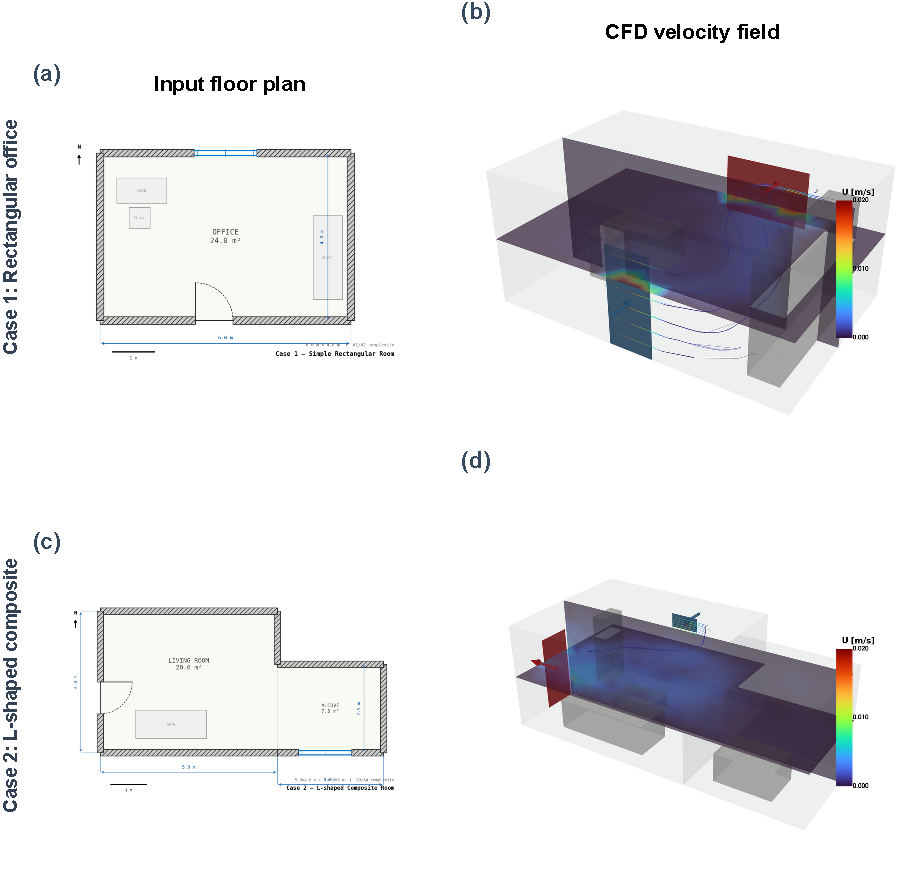
\includegraphics[width=\textwidth]{fig_demo_floorplan_application}
\caption{Application to architectural floor plans. (a,b) Rectangular office (6.0 m $\times$ 4.0 m): input floor plan and CFD velocity field. (c,d) L-shaped room (5.0 m $\times$ 4.0 m + 3.0 m $\times$ 2.5 m alcove): input and CFD result. Both cases converge at 0.18 m mesh resolution.}
\label{fig:demo-floorplan-application}
\end{figure*}

The second case is an L-shaped composite room consisting of a 5.0 m $\times$ 4.0 m living room connected to a 3.0 m $\times$ 2.5 m alcove (Fig.~\ref{fig:demo-floorplan-application}c). The VLM correctly identifies the composite topology as a two-block structure. However, it places four obstacles (a sofa (present in the drawing), a coffee table, a bookshelf, and an alcove desk), of which the latter three are hallucinated and do not appear in the input image. This obstacle hallucination is consistent with the failure mode identified in Section~\ref{sec:discuss-obstacle-hallucination} from the synthetic benchmark. The inlet is assigned to the north wall and the outlet to the west wall. Despite the hallucinated obstacles, the CFD simulation converges and produces a physically plausible flow pattern in which the main jet passes through the living room with a secondary branch entering the alcove region (Fig.~\ref{fig:demo-floorplan-application}d). The scale calibration factor of 0.625 was applied to correct the VLM's initial overestimate of the room dimensions.

Both cases show that the framework tolerates realistic visual noise (hatched walls, furniture icons, dimension lines, door arc symbols) and still converges. The hallucinated obstacles in Case 2 are consistent with the benchmark finding: small spurious obstacles do not disrupt bulk flow patterns. Scale calibration is straightforward when dimension annotations appear on the drawing, which is typical in architectural practice. Floor plan inputs from real drawings are a practical use case for the framework.

\section{Conclusion}
\label{sec:conclusion}


This paper described a framework that converts a single 2D image into an indoor CFD solution by using a VLM for geometric abstraction. Across 100 benchmark cases (four complexity levels, five view types), the framework achieved a mean structural score of 0.781 and a mean CFD agreement score of 0.477 with single-factor scale calibration. The floor-plan view yields the best results, achieving a structural score of 0.884, a CFD agreement score of 0.572, and a 100\% opening-wall match rate. Three characteristic failure modes have been identified and analysed: composite-room collapse under section views, obstacle hallucination with limited CFD penalty, and a structure-versus-fidelity gap in dense configurations. The framework converges for 97 of 100 cases (3 cases fail due to solver divergence from non-physical predicted geometries) through a multi-level robustness strategy.

VLM-based geometric abstraction is adequate for rapid indoor CFD screening when the goal is qualitative flow pattern identification (locating dominant recirculation zones, jet paths, and stagnation regions) rather than precise local velocity magnitudes. For applications requiring high-fidelity local flow prediction near specific obstacles, the current framework's accuracy is insufficient and should be supplemented with manual geometry refinement or multi-view input fusion. Future work will explore multi-factor scale calibration, multi-view input strategies, and extension to transient thermal simulations.


\section*{CRediT authorship contribution statement}


\textbf{Younghwan Joo}: Conceptualization, Methodology, Software, Validation, Formal analysis, Investigation, Data curation, Writing -- original draft, Writing -- review \& editing, Visualization.


\section*{Declaration of competing interest}


The author declares no known competing financial interests or personal relationships that could have appeared to influence the work reported in this paper.


\section*{Data availability}


The benchmark dataset (scene definitions, multi-view renderings, evaluation results), pipeline source code, and evaluation scripts are publicly available on figshare at https://doi.org/10.6084/m9.figshare.31866127.


\section*{Acknowledgements}


This work was conducted under the framework of the research and development program of the Korea Institute of Energy Research (C6-2419-63).



\section{Appendix A. VLM Prompt Template}
\label{sec:appendix-a-vlm-prompt-template}


The full prompt template used for Gemini 3.1 Pro scene extraction (~659 words) is provided as supplementary material. The prompt specifies the `indoor\_cfd\_scene\_v1` JSON schema, the coordinate system convention (origin at room minimum corner, x = west-east, y = south-north, z = floor-ceiling), and solver-stability constraints (no overlapping obstacles, openings within wall bounds, connected fluid domain). When a scale hint is available, an addendum anchors absolute dimensions to a user-provided metric span. The complete prompt text is reproduced in the online supplementary material.

\section{Appendix B. IoU Threshold Sensitivity}
\label{sec:appendix-b-iou-threshold-sensitivity}


The structural score depends on the IoU thresholds used for room-block matching (default 0.2) and obstacle matching (default 0.1). To assess the sensitivity of the reported results to these thresholds, the structural score was recomputed with a uniform IoU threshold applied to both components, ranging from 0.05 to 0.50. Opening type F1 and opening wall match ratio are unaffected by this variation.

\begin{table}[htbp]
\centering
\caption{Mean structural score as a function of uniform IoU matching threshold (n = 97).}
\label{tab:appendix-iou-sensitivity}
\begin{tabular}{ll}
\toprule
IoU threshold & Mean structural score \\
\midrule
0.05 & 0.803 \\
0.10 & 0.783 \\
0.15 & 0.759 \\
0.20 & 0.749 \\
0.30 & 0.710 \\
0.50 & 0.618 \\
\bottomrule
\end{tabular}
\end{table}


The score degrades monotonically from 0.803 at the most lenient threshold to 0.618 at the strictest. The steepest decline occurs between 0.30 and 0.50, indicating that many obstacle and room-block matches fall in the IoU range of 0.3 to 0.5, indicating geometrically reasonable overlap but not tight alignment. The relative ranking of view types and categories is preserved across all thresholds, confirming that the reported conclusions are not artefacts of the particular threshold choice.


\begin{figure*}[htbp]
\centering
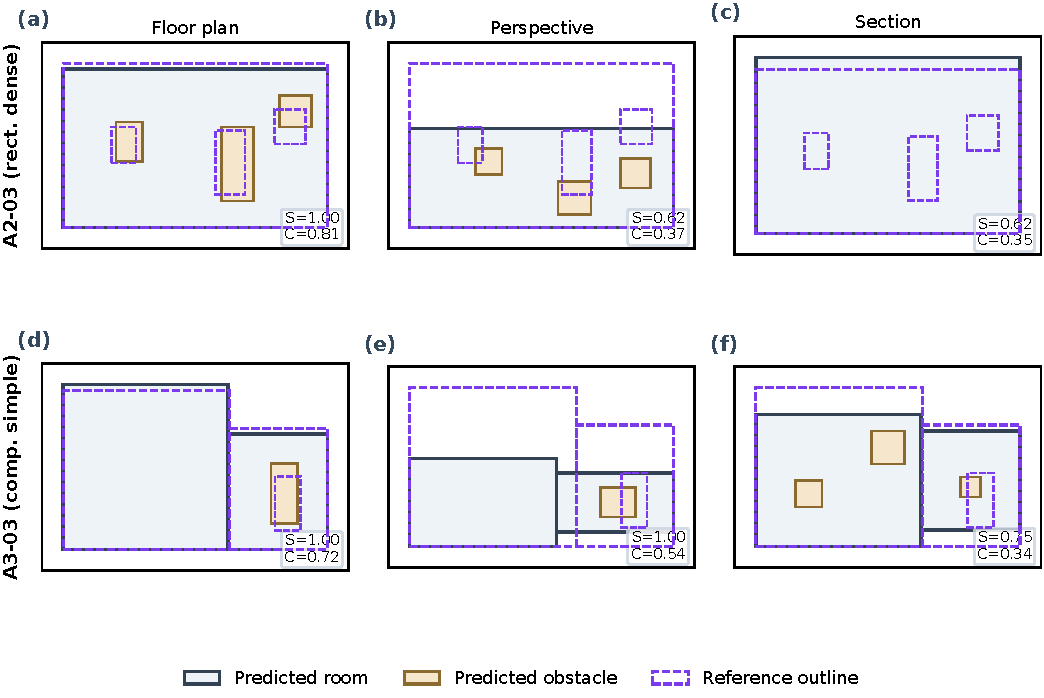
\includegraphics[width=\textwidth]{fig_result_crossview_outcome}
\caption{Cross-view outcome comparison for cases A2-03 and A3-03 across three view types. Matched obstacles are shown in tan, hallucinated obstacles in orange cross-hatch, and reference outlines as dashed purple. Structural (S) and CFD (C) scores are annotated per panel.}
\label{fig:result-crossview-outcome}
\end{figure*}

\begin{figure*}[htbp]
\centering
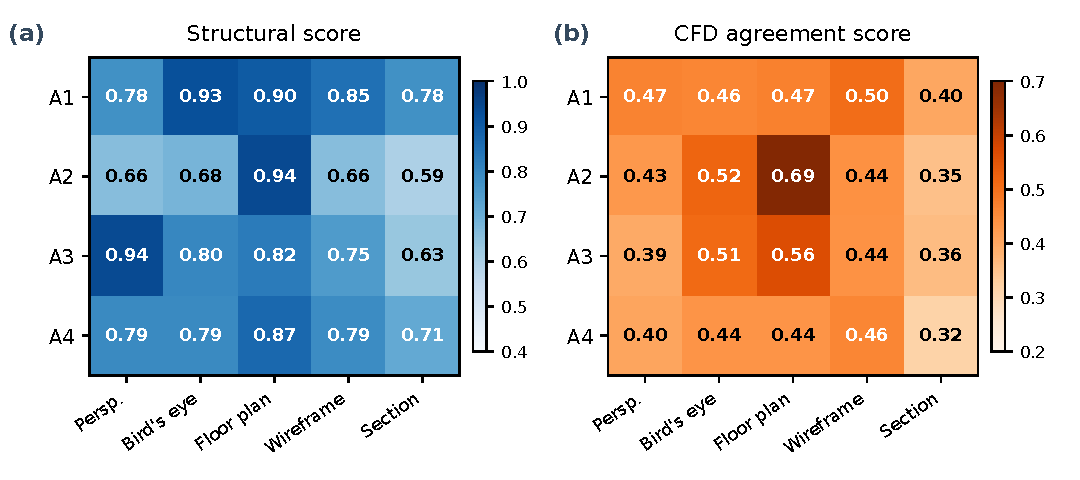
\includegraphics[width=\textwidth]{fig_result_heatmap_category_view}
\caption{Category $\times$ view interaction heatmaps.}
\label{fig:result-heatmap-category-view}
\end{figure*}


\bibliographystyle{elsarticle-num}
\bibliography{Zotero_YHJoo}

\end{document}
